\documentclass[a4paper,12pt]{fancy}
\usepackage{circuitikz}
\usepackage{graphicx}
\graphicspath{ {./images/} }
\usepackage[table]{xcolor}
\usepackage{pdflscape}
\usepackage{adjustbox}
\usepackage{wrapfig}
\usepackage{pdfpages}
\usepackage{physics}
\usepackage[version=4]{mhchem}
\usepackage{pgfplots}
\usetikzlibrary{mindmap} % LATEX and plain TEX
\usetikzlibrary{shadings,shapes.geometric,calc, patterns, angles, quotes, arrows.meta, shapes, decorations.pathmorphing, decorations.shapes, decorations.text, decorations.markings,shadows}
\tikzstyle directed=[postaction={decorate,decoration={markings, % arrows on the field lines
		mark=at position .1 with {\arrowreversed[scale=1.5]{stealth}},
		mark=at position .9 with {\arrowreversed[scale=1.5]{stealth}}}}]
\tikzstyle tangent=[postaction={decorate,decoration={markings, % Tangent to the field line
		mark=at position .7 with {\draw[ultra thick,stealth-,green!60!black,solid](-12pt,0)--(12pt,0)node[above]{$\vec{B}$};}}}]
\tikzstyle fLines=[thick,dashed,directed,tangent]
\tikzset{
	arrow/.style={-{Triangle[length=5mm,width=2mm]}}
}
\tikzset{
	mypath/.style={
		postaction=decorate,
		decoration={markings,
			mark=at position #1 with {\coordinate (x);\arrow{>}}},
		thick},
	>=stealth
}
\pgfdeclareverticalshading{heat}{100bp}{%
	color(0bp)=(white);   color(25bp)=(white); color(30bp)=(cyan!50); 
	color(70bp)=(orange!70); color(75bp)=(white);  color(100bp)=(white)}
\usetikzlibrary{patterns,fillbetween}
\pgfplotsset{width=8cm,compat=newest}
\def\wall{ \fill
	[fill=black!50] (1,-.5) rectangle (2,.5);
	\pattern [pattern=bricks] (1,-.5) rectangle (2,.5);
	\draw
	[line width=1pt] (1cm+.5pt,-.5) -- ++(0,1); }

\begin{document}
%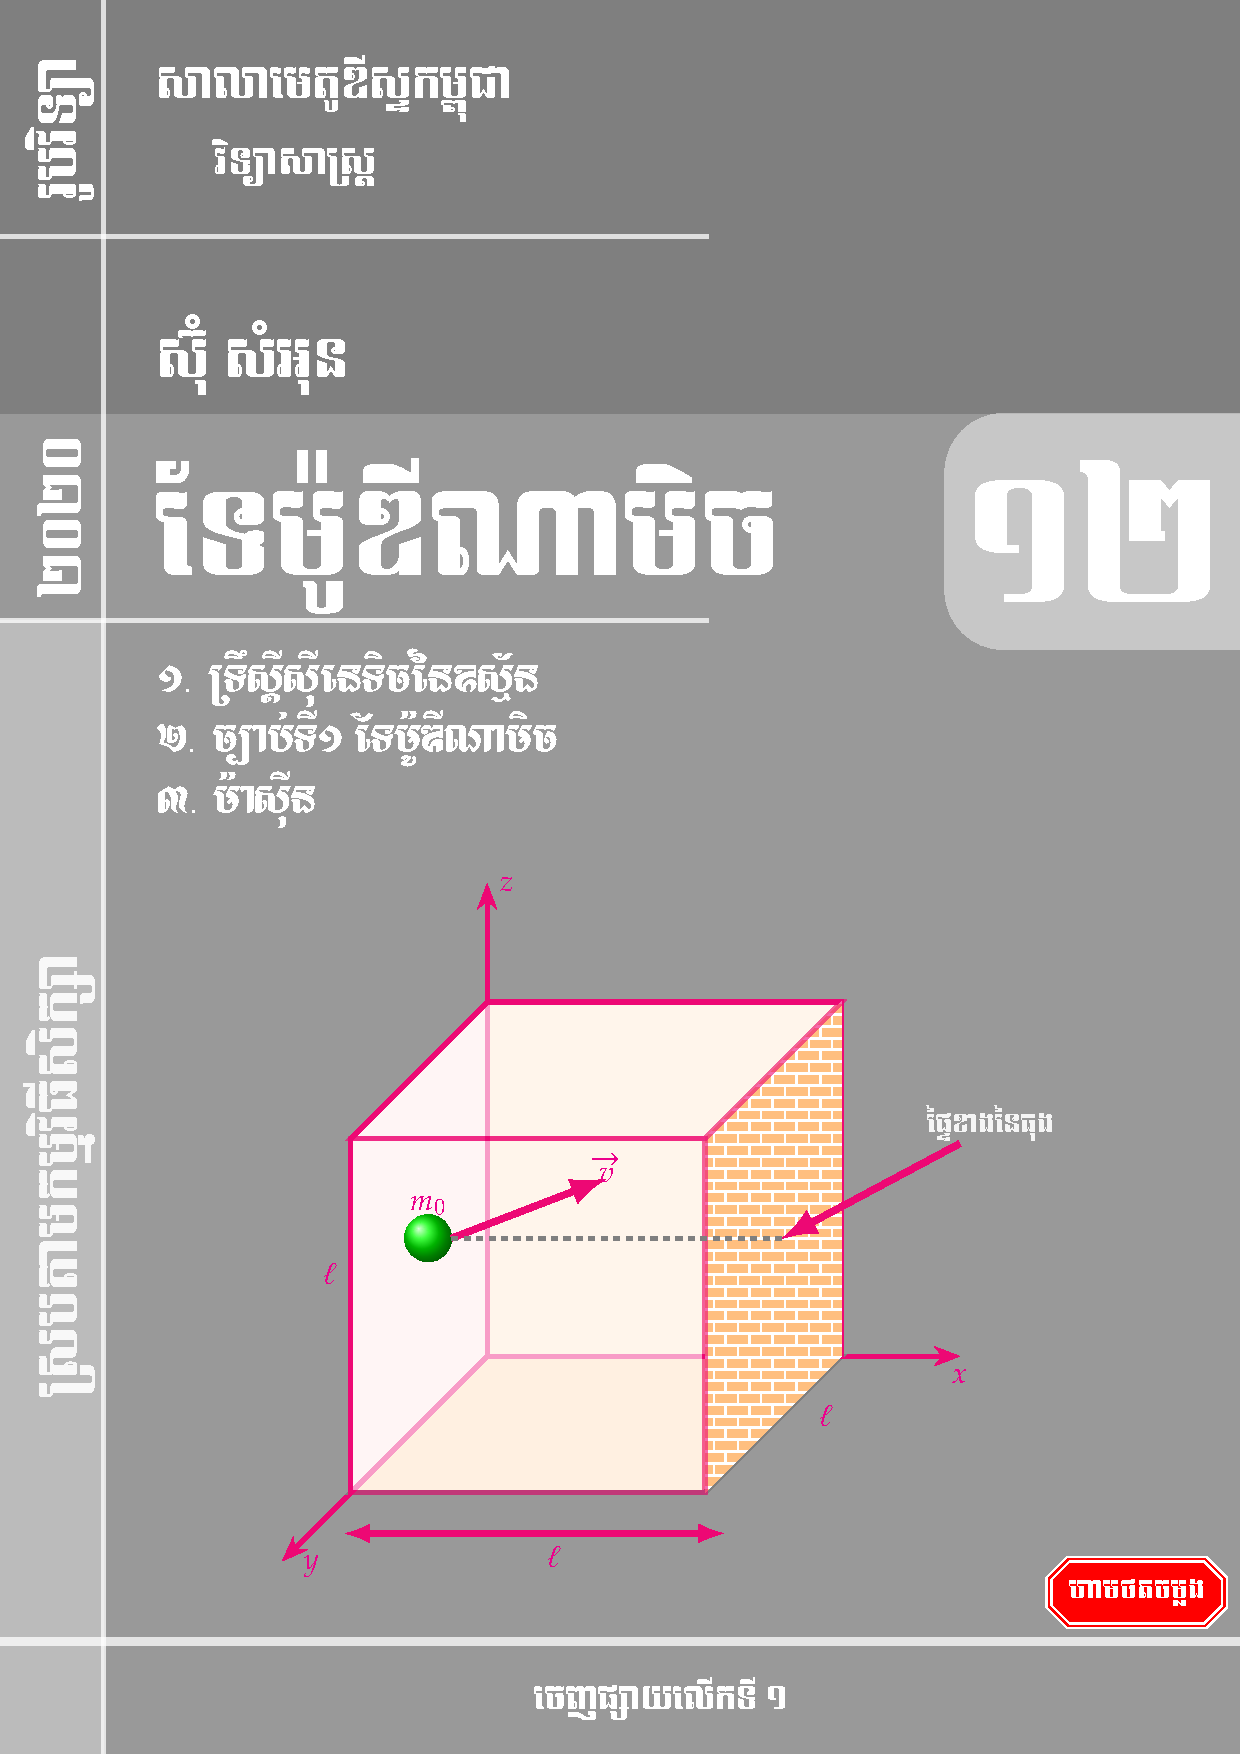
\includepdf[pages=1]{front-cover.pdf}
\frontmatter
\pagenumbering{alpkh}
%\chapter*{សេចក្ដីថ្លែងអំណរគុណ}
\addcontentsline{toc}{chapter}{សេចក្ដីថ្លែងអំណរគុណ}
ខ្ញុំសូមថ្លែងអំណរគុណយ៉ាងជ្រាលជ្រៅដល់មាតាបិតារបស់ខ្ញុំគឺ លោកឪពុក \emph{ឌុច~ទាក់} និង អ្នកម្ដាយ \emph{ឌុក~សារុំ} ដែលបានផ្ដល់អ្វីគ្រប់យ៉ាងដល់រូបខ្ញុំ។ ខ្ញុំសូមថ្លែងអំណរគុណដល់ លោកពូ \emph{ស៊ិន~អ៊ាន} និង អ្នកមីង \emph{ឌុក~សាភូ} ដែលទំនុកបម្រុង ផ្ដល់ដំបូន្មាន និង ការជម្រុញលើកទឹកចិត្ត។ សូមផ្ញើរសេចក្ដីថ្លែងអំណរគុណដល់បងប្អូនខ្ញុំជាច្រើនអ្នកទៀត។
\\[1em]
ជាថ្មីម្ដងទៀតខ្ញុំសូមរំលឹកគុណដល់លោកគ្រូ អ្នកគ្រូរបស់ខ្ញុំដែលបាន បង្ហាត់ពត់លត់ដំខាងផ្នែកបញ្ញាស្មារតី និងវិជ្ជាជីវៈ។ បន្ថែមលើនេះខ្ញុំសូមថ្លែងអំណរគុណដល់មិត្តភ័ក្ដិ និងសិស្សានុសិស្សដែលបានផ្ដល់ជាកំលាំងចិត្តដល់រូបខ្ញុំ។
%\chapter*{អារម្ភកថា}
\addcontentsline{toc}{chapter}{អារម្ភកថា}
កថាខណ្ឌនេះពិពណ៌នាអំពីដំណើរដងទងនៃការចាប់កំណើតឡើងនៃសៀវភៅនេះ។ ដំបូងឡើយវាគ្រាន់តែជាកម្រងលំហាត់សម្រាប់ឲ្យសិស្សអនុវត្តន៏បន្ថែមលើការសិក្សាម៉ោងរដ្ធតែប៉ុណ្ណោះ។ ដោយពេលវេលាមានរយៈពេលខ្លី ការដាក់ឧទាហរណ៏ និងលំហាត់គំរូពុំសូវបានច្រើនជាហេតុបណ្ដាលអោយខ្ញុំកើតគំនិតសរសេរចម្លើយដើម្បីអោយសិស្សអាន និងអនុវត្តន៏ដោយខ្លួនឯង។
\\[1em]
សៀវភៅនេះបែងចែកជាបួនផ្នែករួមមាន មេរៀនសង្ខេបអមដោយឧទាហរណ៏គំរូ កម្រងលំហាត់បញ្ចប់មេរៀន ចម្លើយលំហាត់ និង សេចក្ដីបន្ថែម។ នៅផ្នែកមេរៀនសង្ខេបយើងមាន ការរំលឹកខ្លី និយមន័យ លក្ខណៈ និងទ្រឹស្ដីបទ។ ឧទាហរណ៏គំរូសម្រាប់និយមន័យនីមួយៗ ក៏ត្រូវបានរួមបញ្ចូលនៅផ្នែកនេះដែរ។ សម្រាប់សម្រាយបញ្ជាក់ លក្ខណៈ និងទ្រីស្ដីបទសំខាន់អ្នកអានរកមើលនៅផ្នែកបន្ថែមដែលបានដាក់នៅជំពូកចុងក្រោយគេបង្អស់នៃសៀវភៅ។ នៅផ្នែកកម្រងលំហាត់បញ្ចប់មេរៀន យើងមានតែលំហាត់សុទ្ធដែលត្រូវបានរៀបចំតាមខ្លឹមសារមេរៀន និងតាមលំដាប់កើននៃភាពលំបាក។ បន្ទាប់ពីផ្នែកនេះគឺជាចម្លើយលើកម្រងលំហាត់។ រីឯផ្នែកចុងក្រោយ ជាសេចក្ដីបន្ថែម ដែលភាគច្រើនដកស្រង់ចេញពីមេរៀនថ្នាក់ក្រោម។ អ្នកអានគួរផ្ដោតការយកចិត្តទុកលើផ្នែកនេះជាចំបង។ ផ្នែកនេះគួរតែអានមុនគេដើម្បីបង្កភាពងាយស្រួលក្នុងការអានផ្នែកផ្សេងៗទៀត។
\\[1em]
បញ្ជាក់ជួនដល់អ្នកអានសៀវភៅនេះឲ្យបានជ្រាបថា វាគឺជាស្នារដៃដំបូងរបស់អ្នកនិពន្ធ។ សៀវភៅនេះត្រូវបានបង្កើតឡើងដោយមនុស្សតែម្នាក់ប៉ុណ្ណោះ។ ជាងនេះទៅទៀតវាពុំទាន់បានឆ្លងកាត់ការត្រួតពិនិត្យទាំងផ្នែកបច្ចេកទេស និងអក្ខរាវិរុទ នៅឡើយទេ។ បើប្រិយមិត្តរកឃើញកំហុសឆ្គងណាមួយ សូមជួនដំណឹងដល់អ្នកសរសេរសៀវភៅដោយការផ្ញើរសារជាអក្សរ ឬ រូបភាពមកកាន់ប្រអប់សារអេឡិចត្រូនិច ដែលមានអាស័យដ្ឋាន \textcolor{magenta}{\itshape bunnybookauthor@gmail.com} បើមិនអញ្ចឹងទេអ្នកអាចជួបពិភាក្សាផ្ទាល់បើអាចធ្វើទៅបាន។
\\[1em]
ទាក់ទិននឹងការធ្វើអាជីវកម្មលើសៀវភៅនេះ អ្នកនិពន្ធរក្សាសិទ្ធិកម្មសិទ្ធិបញ្ញាដោយមិនអនុញ្ញាតអោយធ្វើការបោះពុម្ភ ថតចំលង ឬចែកចាយដោយគ្មានការអនុញ្ញាតឡើយ។ ចំពោះកំណាត់សៀវភៅនេះជាឯកសារអេឡិចត្រូនិច អ្នកអាចទាញយកមកអាន និងប្រើប្រាស់ផ្ទាល់ខ្លួនបានដោយមិនគិតថ្លៃតាមរយៈដំណរ\\ \textcolor{magenta}{\itshape bunnybookshelf.blogspot.com/p/conic.html}~។
\clearpage
\tableofcontents
\addcontentsline{toc}{chapter}{\contentsname}
\mainmatter
\pagenumbering{khmer}
\chapter{ចំនួនអសនិទាន}
\section{ឬសការេ}
\begin{generality}
បើ $a>0,\quad x^2=a$ គេបាន $x=\sqrt{a}$ និង  $x=-\sqrt{a}$។
\end{generality}

\section{ឬសគួប}
\begin{generality}
បើ $ x^3=a$ គេបាន $x=\sqrt[3]{a},\quad a$ អាចវិជ្ជមាន ឬ អវិជ្ជមាន ។
\end{generality}

\section{ប្រមាណវិធីលើរ៉ាឌីកាល់}
\subsection{វិធីគុណ}
\begin{generality}
ផលគុណនៃរ៉ាឌីកាល់ដែលមានសន្ទស្សន៍ដូចគ្នាស្មើនឹងរ៉ាឌីកាល់នៃផលគុណ
\begin{enumerate}[label=\alph*.]
	\item $\sqrt{a}\cdot \sqrt{b}=\sqrt{ab},\quad a\ge 0,b\ge 0$
	\item $\sqrt[3]{a}\cdot \sqrt[3]{b}=\sqrt[3]{ab}\quad a,b$ អាចជាចំនួនវិជ្ជមានឬអវិជ្ជមាន។
\end{enumerate}
\end{generality}
\subsection{វិធីចែក}
\begin{generality}
ផលចែកនៃរ៉ាឌីកាល់ដែលមានសន្ទស្សន៍ដូចគ្នាស្មើនឹងរ៉ាឌីកាល់នៃផលចែក
\begin{enumerate}[label=\alph*.]
	\item $\dfrac{\sqrt{a}}{\sqrt{b}}=\sqrt{\dfrac{a}{b}},\quad a\ge 0,b> 0$
	\item $\dfrac{\sqrt[3]{a}}{\sqrt[3]{b}}=\sqrt[3]{\dfrac{a}{b}},\quad ,b\ne 0$
\end{enumerate}
\end{generality}
\subsection{ការបញ្ចេញមួយចំនួនពីក្នុងរ៉ាឌីកាល់}
\begin{generality}
ដើម្បីបញ្ចេញមួយចំនួនពីរ៉ាឌីកាល់ គេត្រូវបំប្លែងរ៉ាឌីកង់ជាស្វ័យគុណដែលមាននិទស្សន្តស្មើនឹងសន្ទស្សន៍នៃរ៉ាឌីកាល់។
\end{generality}

\subsection{កាបញ្ចូលមួយចំនួនទៅក្នុងរ៉ាឌីកាល់}
\begin{generality}
ដើម្បីបញ្ចេញមួយចំនួនទៅក្នុងរ៉ាឌីកាល់ គេត្រូវលើកចំនួននោះជាស្វ័យគុណដោយឲ្យនិទស្សន្តនៃស្វ័យគុណស្មើនឹងសន្ទស្សន៍នៃរ៉ាឌីកាល់។
\end{generality}
\subsection{វិធីបូក និង វិធីដក}

\begin{generality}
ដើម្បីគណនាផលបូក និង ផលដករ៉ាឌីកាល់ដែលមានសន្ទស្សន៍ដូចគ្នាគេត្រូវបំប្លែងរ៉ាឌីកង់ឲ្យដូចគ្នា។ 
ដើម្បីគណនាផលបូក និង ផលដករ៉ាឌីកាល់ដែលមានសន្ទស្សន៍ដូចគ្នា និង មានសន្ទស្សន៍ដូចគ្នា គេបូក-ដកមេគុណនឹងមេគុណ ហើយរ៉ាឌីកាល់ទុកដដែល។
\end{generality}
%%%%%%%%%%%%%%%%%%%%%%%%%%%%%%%%%%%%%%%%%%%%%%
\newpage
\section{ផ្នែកលំហាត់មានដំណោះស្រាយ}
\begin{center}
ចូរជ្រើសរើសចម្លើយដែលមានតែមួយគត់ នៅក្នុងសំណួរនីមួយៗខាងក្រោម៖
\end{center}
\begin{enumerate}
%P1
\item តម្លៃ $x$ ដែលផ្ទៀងផ្ទាត់សមីការ $2x+3=5$ គឺ
\begin{enumerate}[k,4]
	\item $x=1$
	\item $x=-1$
	\item $x=2$
	\item $x=-2$
\end{enumerate}

%P2
\item តម្លៃ $x$ ដែលផ្ទៀងផ្ទាត់សមីការ $-2x+3=5$ គឺ
\begin{enumerate}[k,4]
	\item $x=1$
	\item $x=-1$
	\item $x=2$
	\item $x=-2$
\end{enumerate}

%P3
\item តម្លៃ $x$ ដែលផ្ទៀងផ្ទាត់សមីការ $(x+1)(x+2)=x^2+5$ គឺ
\begin{enumerate}[k,4]
	\item $x=1$
	\item $x=-1$
	\item $x=2$
	\item $x=-2$
\end{enumerate}

%P4
\item កន្សោម$A=x^2-4$ អាចសរសេរជាទម្រង់៖
\begin{enumerate}[k,4]
	\item $A=(x+2)^2$
	\item $A=(x-2)^2$
	\item $A=(x+2)(x+2)$
	\item $A=(x-2)(x+2)$
\end{enumerate}

%P5
\item សមីការ $x^2-4=0$ មានចម្លើយវិជ្ជមានមួយគត់គឺ៖
\begin{enumerate}[k,4]
	\item $x=-4$
	\item $x=4$
	\item $x=2$
	\item $x=-2$
\end{enumerate}

%P6
\item តម្លៃ $x$ ដែលផ្ទៀងផ្ទាត់សមភាព $x^2=25$ គឺ៖
\begin{enumerate}[k,4]
	\item $x=-\sqrt{5}$
	\item $x=\sqrt{5}$
	\item $x=5$
	\item $x=-5$
\end{enumerate}

%P7
\item តម្លៃ $x$ ដែលផ្ទៀងផ្ទាត់សមភាព $x^2=49$ គឺ៖
\begin{enumerate}[k,4]
	\item $x=-\sqrt{7}$
	\item $x=\sqrt{7}$
	\item $x=7$
	\item $x=-7$
\end{enumerate}

%P8
\item តម្លៃនៃកន្សោម $A=\sqrt{64}$  គឺ៖
\begin{enumerate}[k,4]
	\item $x=-8,8$
	\item $x=-8$
	\item $x=8$
	\item $x=4$
\end{enumerate}

%P9
\item តម្លៃនៃកន្សោម $A=-\sqrt{64}$  គឺ៖
\begin{enumerate}[k,4]
	\item $x=-8,8$
	\item $x=-8$
	\item $x=8$
	\item $x=4$
\end{enumerate}

%P10
\item តម្លៃនៃកន្សោម $A=\sqrt{\left(1-\sqrt{3}\right)^2}$  គឺ៖
\begin{enumerate}[k,4]
	\item $x=1-\sqrt{3}$
	\item $x=-1-\sqrt{3}$
	\item $x=1+\sqrt{3}$
	\item $x=-1+\sqrt{3}$
\end{enumerate}

%P11
\item សមីការ $x^2=0$ មានឬសគឺ៖
\begin{enumerate}[k,4]
	\item $x=2$
	\item $x=-2$
	\item $x=0$
	\item $x=-1$
\end{enumerate}

%P12
\item សមីការ $x^2=-4$ មានឬសគឺ៖
\begin{enumerate}[k,4]
	\item $x=2$
	\item $x=-2$
	\item សមីការមានចម្លើយមួយ
	\item សមីការគ្មានចម្លើយ
\end{enumerate}

%P13
\item សមីការ $x^2=\dfrac{25}{4}$ មានឬសអវិជ្ជមានមួយគឺ៖
\begin{enumerate}[k,4]
	\item $x=-2$
	\item $x=-5$
	\item $x=-\dfrac{5}{2}$
	\item $x=\pm \dfrac{5}{2}$
\end{enumerate}

%P14
\item សមីការ $x^2-1=80$ មានឬសគឺ៖
\begin{multicols}{4}
\begin{enumerate}[label=\alph*.]
	\item $x=-9$
	\item $x=-8$
	\item $x=\pm 9$
	\item $x=\pm 8$
\end{enumerate}
\end{multicols}

%P15
\item សមីការ $x^2=0.01$ មានឬសគឺ៖
\begin{multicols}{4}
\begin{enumerate}[label=\alph*.]
	\item $x=0.001$
	\item $x=-0.001$
	\item $x=\pm 0.1$
	\item $x=\pm 0.2$
\end{enumerate}
\end{multicols}

%P16
\item សមីការ $x^2=\dfrac{1}{36}$ មានឬសគឺ៖
\begin{multicols}{4}
\begin{enumerate}[label=\alph*.]
	\item $x=-6$
	\item $x=6$
	\item $x=\dfrac{1}{6}$
	\item $x=\pm \dfrac{1}{6}$
\end{enumerate}
\end{multicols}

%P17
\item សមីការ $x^2=3$ មានឬសគឺ៖
\begin{multicols}{4}
\begin{enumerate}[label=\alph*.]
	\item $x=-3$
	\item $x=3$
	\item $x=\sqrt{3}$
	\item $x=\pm \sqrt{3}$
\end{enumerate}
\end{multicols}

%P18
\item សមីការ $x^2=625$ មានឬសគឺ៖
\begin{multicols}{4}
\begin{enumerate}[label=\alph*.]
	\item $x=-15$
	\item $x=\pm 15$
	\item $x=-25$
	\item $x=\pm 25$
\end{enumerate}
\end{multicols}

%P19
\item សមីការ $x^2=-1225$ មានឬសគឺ៖
\begin{multicols}{4}
\begin{enumerate}[label=\alph*.]
	\item $x=-35$
	\item $x=35$
	\item $x=\pm \sqrt{-1225}$
	\item គ្មានចម្លើយ
\end{enumerate}
\end{multicols}

%P20
\item សមីការ $x^2=-225$ មានឬសគឺ៖
\begin{multicols}{4}
\begin{enumerate}[label=\alph*.]
	\item $x=-15$
	\item $x=15$
	\item $x=\pm \sqrt{-1225}$
	\item គ្មានចម្លើយ
\end{enumerate}
\end{multicols}

%P21
\item ចូរសរសេរតម្លៃនៃ$8$ ជាទម្រង់ផលគុណកត្តាបឋម៖
\begin{multicols}{4}
\begin{enumerate}[label=\alph*.]
	\item $2\times 4$
	\item $1\times 8$
	\item $2\times 2\times 3$
	\item $2\times 2\times 2$
\end{enumerate}
\end{multicols}

%P22
\item ចូរសរសេរតម្លៃនៃ$210$ ជាទម្រង់ផលគុណកត្តាបឋម៖
\begin{multicols}{4}
\begin{enumerate}[label=\alph*.]
	\item $21\times 10$
	\item $42 \times 5$
	\item $21\times 2\times 5$
	\item $2\times 3\times 5\times 7$
\end{enumerate}
\end{multicols}

%P23
\item ចូរសរសេរតម្លៃនៃ$32$ ជាទម្រង់ផលគុណកត្តាបឋម៖
\begin{multicols}{4}
\begin{enumerate}[label=\alph*.]
	\item $16\times 2$
	\item $8 \times 4$
	\item $2^5+1$
	\item $2^5$
\end{enumerate}
\end{multicols}
%P24
\item ចូរសរសេរតម្លៃនៃ$250$ ជាទម្រង់ផលគុណកត្តាបឋម៖
\begin{multicols}{4}
\begin{enumerate}[label=\alph*.]
	\item $25\times 10$
	\item $125\times 2$
	\item $50\times 5$
	\item $2\times 5^3$
\end{enumerate}
\end{multicols}
%P25
\item ចូរសរសេរតម្លៃនៃ$54$ ជាទម្រង់ផលគុណកត្តាបឋម៖
\begin{multicols}{4}
\begin{enumerate}[label=\alph*.]
	\item $27\times 2$
	\item $9\times 6$
	\item $18\times 3$
	\item $2\times 3^3$
\end{enumerate}
\end{multicols}

%P26
\item តម្លៃ $x$ ដែលផ្ទៀងផ្ទាត់សមីការ $x^3=8$គឺ៖
\begin{multicols}{4}
\begin{enumerate}[label=\alph*.]
	\item $x=-2$
	\item $x=2$
	\item $x=\pm 2$
	\item គ្មានតម្លៃ$x$
\end{enumerate}
\end{multicols}

%P27
\item តម្លៃ $x$ ដែលផ្ទៀងផ្ទាត់សមីការ $x^3=27$គឺ៖
\begin{multicols}{4}
\begin{enumerate}[label=\alph*.]
	\item $x=-3$
	\item $x=3$
	\item $x=\pm 3$
	\item $x=0$
\end{enumerate}
\end{multicols}

%P28
\item តម្លៃ $x$ ដែលផ្ទៀងផ្ទាត់សមីការ $x^3=-27$គឺ៖
\begin{multicols}{4}
\begin{enumerate}[label=\alph*.]
	\item $x=-3$
	\item $x=3$
	\item $x=\pm 3$
	\item $x=0$
\end{enumerate}
\end{multicols}

%P29
\item តម្លៃ $x$ ដែលផ្ទៀងផ្ទាត់សមីការ $x^3=64$គឺ៖
\begin{multicols}{4}
\begin{enumerate}[label=\alph*.]
	\item $x=4$
	\item $x=-4$
	\item $x=\pm 4$
	\item $x=\pm 8$
\end{enumerate}
\end{multicols}

%P30
\item តម្លៃ $x$ ដែលផ្ទៀងផ្ទាត់សមីការ $x^3=125$គឺ៖
\begin{multicols}{4}
\begin{enumerate}[label=\alph*.]
	\item $x=15$
	\item $x=-15$
	\item $x=\pm 5$
	\item $x=5$
\end{enumerate}
\end{multicols}

%P31
\item តម្លៃ $x$ ដែលផ្ទៀងផ្ទាត់សមីការ $x^3+125=0$គឺ៖
\begin{multicols}{4}
\begin{enumerate}[label=\alph*.]
	\item $x=15$
	\item $x=-15$
	\item $x=-5$
	\item $x=5$
\end{enumerate}
\end{multicols}

%P32
\item តម្លៃ $x$ ដែលផ្ទៀងផ្ទាត់សមីការ $x^3-1=215$គឺ៖
\begin{multicols}{4}
\begin{enumerate}[label=\alph*.]
	\item $x=16$
	\item $x=-16$
	\item $x=-6$
	\item $x=6$
\end{enumerate}
\end{multicols}

%P33
\item តម្លៃ $x$ ដែលផ្ទៀងផ្ទាត់សមីការ $x^3=-216$គឺ៖
\begin{multicols}{4}
\begin{enumerate}[label=\alph*.]
	\item $x=16$
	\item $x=-16$
	\item $x=-6$
	\item $x=6$
\end{enumerate}
\end{multicols}
%P34
\item តម្លៃ $x$ ដែលផ្ទៀងផ្ទាត់សមីការ $x^3=\dfrac{1}{8}$គឺ៖
\begin{multicols}{4}
\begin{enumerate}[label=\alph*.]
	\item $x=\dfrac{1}{2}$
	\item $x=-\dfrac{1}{2}$
	\item $x=-2$
	\item $x=2$
\end{enumerate}
\end{multicols}

%P35
\item តម្លៃ $x$ ដែលផ្ទៀងផ្ទាត់សមីការ $x^3=0.008$គឺ៖
\begin{multicols}{4}
\begin{enumerate}[label=\alph*.]
	\item $x=\dfrac{1}{2}$
	\item $x=-\dfrac{1}{2}$
	\item $x=-0.2$
	\item $x=0.2$
\end{enumerate}
\end{multicols}
%P36
\item តម្លៃ $x$ ដែលផ្ទៀងផ្ទាត់សមីការ $x^3=0.125$គឺ៖
\begin{multicols}{4}
\begin{enumerate}[label=\alph*.]
	\item $x=\dfrac{1}{5}$
	\item $x=-\dfrac{1}{5}$
	\item $x=-0.5$
	\item $x=0.5$
\end{enumerate}
\end{multicols}

%P37
\item តម្លៃ $x$ ដែលផ្ទៀងផ្ទាត់សមីការ $x^3=-0.216$គឺ៖
\begin{multicols}{4}
\begin{enumerate}[label=\alph*.]
	\item $x=\dfrac{1}{6}$
	\item $x=-\dfrac{1}{6}$
	\item $x=-0.6$
	\item $x=0.6$
\end{enumerate}
\end{multicols}

%P38
\item តម្លៃ $x$ ដែលផ្ទៀងផ្ទាត់សមីការ $x^3=9$គឺ៖
\begin{multicols}{4}
\begin{enumerate}[label=\alph*.]
	\item $x=3$
	\item $x=-3$
	\item $x=\sqrt{3}$
	\item $x=\sqrt[3]{9}$
\end{enumerate}
\end{multicols}

%P39
\item តម្លៃ $x$ ដែលផ្ទៀងផ្ទាត់សមីការ $x^3=1331$គឺ៖
\begin{multicols}{4}
\begin{enumerate}[label=\alph*.]
	\item $x=121$
	\item $x=-11$
	\item $x=11$
	\item $x=-121$
\end{enumerate}
\end{multicols}

%P40
\item អាងទឹកមួយមានរាងជាគូបដែលមានជ្រុងប្រវែង$1m$ គណនាចំណុះទឹកដែលអាងនោះអាចស្តុកបាន៖
\begin{multicols}{4}
\begin{enumerate}[label=\alph*.]
	\item $100l$
	\item $100m^3$
	\item $10l$
	\item $1000l$
\end{enumerate}
\end{multicols}

%P41
\item កំណត់ចំនួនគត់វិជ្ជមាន $n$ តូចបំផុតដែលធ្វើអោយ $\sqrt[3]{32n}$ ជាចំនួនគត់៖
\begin{multicols}{4}
\begin{enumerate}[label=\alph*.]
	\item $n=1$
	\item $n=2$
	\item $n=3$
	\item $n=4$
\end{enumerate}
\end{multicols}

%P42
\item ផលគុណនៃកន្សោម$A=\sqrt{2}\times \sqrt{8}$  មានតម្លៃស្មើនឹង៖
\begin{multicols}{4}
\begin{enumerate}[label=\alph*.]
	\item $A=2$
	\item $A=3$
	\item $A=4$
	\item $A=5$
\end{enumerate}
\end{multicols}
%P43
\item ផលគុណនៃកន្សោម$A=\sqrt{3}\times \sqrt{27}$  មានតម្លៃស្មើនឹង៖
\begin{multicols}{4}
\begin{enumerate}[label=\alph*.]
	\item $A=-9$
	\item $A=3$
	\item $A=9$
	\item $A=5$
\end{enumerate}
\end{multicols}

%P44
\item ផលគុណនៃកន្សោម$A=\sqrt[3]{2}\times \sqrt[3]{8}$  មានតម្លៃស្មើនឹង៖
\begin{multicols}{4}
\begin{enumerate}[label=\alph*.]
	\item $A=2$
	\item $A=3$
	\item $A=4$
	\item $A=5$
\end{enumerate}
\end{multicols}
%P45
\item ផលគុណនៃកន្សោម$A=\sqrt[3]{2}\times \sqrt[3]{\frac{1}{16}}$  មានតម្លៃស្មើនឹង៖
\begin{multicols}{4}
\begin{enumerate}[label=\alph*.]
	\item $A=2$
	\item $A=\frac{1}{2}$
	\item $A=4$
	\item $A=-\frac{1}{2}$
\end{enumerate}
\end{multicols}

%P46
\item ផលគុណនៃកន្សោម$A=\sqrt{2}\times \sqrt{32}$  មានតម្លៃស្មើនឹង៖
\begin{multicols}{4}
\begin{enumerate}[label=\alph*.]
	\item $A=-9$
	\item $A=3$
	\item $A=9$
	\item $A=5$
\end{enumerate}
\end{multicols}

%P47
\item ផលគុណនៃកន្សោម$A=\sqrt{50}\times \sqrt{2}$  មានតម្លៃស្មើនឹង៖
\begin{multicols}{4}
\begin{enumerate}[label=\alph*.]
	\item $A=-9$
	\item $A=3$
	\item $A=9$
	\item $A=10$
\end{enumerate}
\end{multicols}

%P48
\item ផលគុណនៃកន្សោម$A=\sqrt{0.1}\times \sqrt{10}$  មានតម្លៃស្មើនឹង៖
\begin{multicols}{4}
\begin{enumerate}[label=\alph*.]
	\item $A=-1$
	\item $A=1$
	\item $A=-2$
	\item $A=2$
\end{enumerate}
\end{multicols}

%P49
\item ផលគុណនៃកន្សោម$A=\sqrt[3]{0.1}\times \sqrt[3]{10}$  មានតម្លៃស្មើនឹង៖
\begin{multicols}{4}
\begin{enumerate}[label=\alph*.]
	\item $A=-1$
	\item $A=1$
	\item $A=-2$
	\item $A=2$
\end{enumerate}
\end{multicols}

%P50
\item ផលចែកនៃកន្សោម$A=\dfrac{\sqrt{8}}{\sqrt{2}}$  មានតម្លៃស្មើនឹង៖
\begin{multicols}{4}
\begin{enumerate}[label=\alph*.]
	\item $A=-1$
	\item $A=1$
	\item $A=-2$
	\item $A=2$
\end{enumerate}
\end{multicols}

%P51
\item ផលចែកនៃកន្សោម$A=\dfrac{\sqrt{288}}{\sqrt{2}}$  មានតម្លៃស្មើនឹង៖
\begin{multicols}{4}
\begin{enumerate}[label=\alph*.]
	\item $A=10$
	\item $A=12$
	\item $A=-12$
	\item $A=22$
\end{enumerate}
\end{multicols}

%P52
\item ផលចែកនៃកន្សោម$A=\dfrac{\sqrt{27}}{\sqrt{3}}$  មានតម្លៃស្មើនឹង៖
\begin{multicols}{4}
\begin{enumerate}[label=\alph*.]
	\item $A=-3$
	\item $A=3$
	\item $A=-4$
	\item $A=4$
\end{enumerate}
\end{multicols}

%P53
\item ផលចែកនៃកន្សោម$A=\dfrac{\sqrt{10}}{\sqrt{0.1}}$  មានតម្លៃស្មើនឹង៖
\begin{multicols}{4}
\begin{enumerate}[label=\alph*.]
	\item $A=-10$
	\item $A=10$
	\item $A=-2$
	\item $A=2$
\end{enumerate}
\end{multicols}

%P54
\item ផលចែកនៃកន្សោម$A=\dfrac{\sqrt[3]{48}}{\sqrt[3]{6}}$  មានតម្លៃស្មើនឹង៖
\begin{multicols}{4}
\begin{enumerate}[label=\alph*.]
	\item $A=-10$
	\item $A=10$
	\item $A=-2$
	\item $A=2$
\end{enumerate}
\end{multicols}
%P55
\item ផលចែកនៃកន្សោម$A=\dfrac{\sqrt[3]{16}}{\sqrt[3]{2}}$  មានតម្លៃស្មើនឹង៖
\begin{multicols}{4}
\begin{enumerate}[label=\alph*.]
	\item $A=-10$
	\item $A=10$
	\item $A=-2$
	\item $A=2$
\end{enumerate}
\end{multicols}

%P56
\item ផលចែកនៃកន្សោម$A=\dfrac{\sqrt[3]{25}}{\sqrt[3]{0.2}}$  មានតម្លៃស្មើនឹង៖
\begin{multicols}{4}
\begin{enumerate}[label=\alph*.]
	\item $A=-5$
	\item $A=5$
	\item $A=-2$
	\item $A=2$
\end{enumerate}
\end{multicols}

%P57
\item ផលចែកនៃកន្សោម$A=\dfrac{\sqrt[3]{\frac{1}{2}}}{\sqrt[3]{4}}$  មានតម្លៃស្មើនឹង៖
\begin{multicols}{4}
\begin{enumerate}[label=\alph*.]
	\item $A=-\dfrac{1}{2}$
	\item $A=\dfrac{1}{2}$
	\item $A=-2$
	\item $A=2$
\end{enumerate}
\end{multicols}
%P58
\item ផលចែកនៃកន្សោម$A=\dfrac{\sqrt[3]{100}}{\sqrt[3]{0.1}}$  មានតម្លៃស្មើនឹង៖
\begin{multicols}{4}
\begin{enumerate}[label=\alph*.]
	\item $A=-\dfrac{1}{10}$
	\item $A=\dfrac{1}{10}$
	\item $A=-10$
	\item $A=10$
\end{enumerate}
\end{multicols}

%P59
\item ផលចែកនៃកន្សោម$A=\dfrac{\sqrt{7}}{\sqrt{28}}$  មានតម្លៃស្មើនឹង៖
\begin{multicols}{4}
\begin{enumerate}[label=\alph*.]
	\item $A=-\dfrac{1}{2}$
	\item $A=\dfrac{1}{2}$
	\item $A=-2$
	\item $A=2$
\end{enumerate}
\end{multicols}
%P60
\item ផលចែកនៃកន្សោម$A=\dfrac{\sqrt[3]{128}}{\sqrt[3]{2}}$  មានតម្លៃស្មើនឹង៖
\begin{multicols}{4}
\begin{enumerate}[label=\alph*.]
	\item $A=-\dfrac{1}{4}$
	\item $A=\dfrac{1}{4}$
	\item $A=-4$
	\item $A=4$
\end{enumerate}
\end{multicols}

%P61
\item តម្លៃនៃកន្សោម $A=\sqrt{\frac{2}{8}}$ មានតម្លៃស្មើនឹង៖
\begin{multicols}{4}
\begin{enumerate}[label=\alph*.]
	\item $A=-\dfrac{1}{2}$
	\item $A=\dfrac{1}{2}$
	\item $A=-2$
	\item $A=2$
\end{enumerate}
\end{multicols}

%P62
\item តម្លៃនៃកន្សោម $A=\sqrt[3]{\frac{81}{3}}$ មានតម្លៃស្មើនឹង៖
\begin{multicols}{4}
\begin{enumerate}[label=\alph*.]
	\item $A=-\dfrac{1}{3}$
	\item $A=\dfrac{1}{3}$
	\item $A=-3$
	\item $A=3$
\end{enumerate}
\end{multicols}

%P63
\item តម្លៃនៃកន្សោម $A=\sqrt{12}$ មានតម្លៃស្មើនឹង៖
\begin{multicols}{4}
\begin{enumerate}[label=\alph*.]
	\item $A=-3\sqrt{3}$
	\item $A=3\sqrt{2}$
	\item $A=-2\sqrt{3}$
	\item $A=2\sqrt{3}$
\end{enumerate}
\end{multicols}

%P64
\item តម្លៃនៃកន្សោម $A=\sqrt[3]{81}$ មានតម្លៃស្មើនឹង៖
\begin{multicols}{4}
\begin{enumerate}[label=\alph*.]
	\item $A=3\sqrt{3}$
	\item $A=3\sqrt[3]{3}$
	\item $A=-2\sqrt[3]{3}$
	\item $A=2\sqrt[3]{3}$
\end{enumerate}
\end{multicols}

%P65
\item តម្លៃនៃកន្សោម $A=\sqrt{50}$ មានតម្លៃស្មើនឹង៖
\begin{multicols}{4}
\begin{enumerate}[label=\alph*.]
	\item $A=4\sqrt{2}$
	\item $A=-5\sqrt{2}$
	\item $A=5\sqrt{2}$
	\item $A=-5\sqrt{3}$
\end{enumerate}
\end{multicols}

%P66
\item តម្លៃនៃកន្សោម $A=\sqrt{\dfrac{2}{25}}$ មានតម្លៃស្មើនឹង៖
\begin{multicols}{4}
\begin{enumerate}[label=\alph*.]
	\item $A=\dfrac{2}{5}$
	\item $A=\dfrac{\sqrt{2}}{5}$
	\item $A=-\dfrac{\sqrt{2}}{5}$
	\item $A=-\dfrac{2}{5}$
\end{enumerate}
\end{multicols}

%P67
\item តម្លៃនៃកន្សោម $A=\dfrac{2}{3}\sqrt{\dfrac{12}{5}}$ មានតម្លៃស្មើនឹង៖
\begin{multicols}{4}
\begin{enumerate}[label=\alph*.]
	\item $A=\sqrt{\dfrac{16}{15}}$
	\item $A=\sqrt{\dfrac{25}{16}}$
	\item $A=-\sqrt{\dfrac{16}{15}}$
	\item $A=\sqrt{\dfrac{8}{15}}$
\end{enumerate}
\end{multicols}

%P68
\item តម្លៃនៃកន្សោម $A=5\sqrt{\dfrac{3}{50}}$ មានតម្លៃស្មើនឹង៖
\begin{multicols}{4}
\begin{enumerate}[label=\alph*.]
	\item $A=\sqrt{\dfrac{3}{4}}$
	\item $A=\sqrt{\dfrac{3}{25}}$
	\item $A=\sqrt{\dfrac{3}{2}}$
	\item $A=\sqrt{\dfrac{6}{25}}$
\end{enumerate}
\end{multicols}

%P69
\item តម្លៃនៃកន្សោម $A=-7\sqrt{5}$ មានតម្លៃស្មើនឹង៖
\begin{multicols}{4}
\begin{enumerate}[label=\alph*.]
	\item $A=\sqrt{245}$
	\item $A=\sqrt{235}$
	\item $A=\sqrt{225}$
	\item $A=\sqrt{215}$
\end{enumerate}
\end{multicols}

%P70
\item តម្លៃនៃកន្សោម $A=-5\sqrt[3]{\dfrac{4}{25}}$ មានតម្លៃស្មើនឹង៖
\begin{multicols}{4}
\begin{enumerate}[label=\alph*.]
	\item $A=-\sqrt[3]{10}$
	\item $A=-\sqrt[3]{20}$
	\item $A=\sqrt[3]{10}$
	\item $A=\sqrt[3]{20}$
\end{enumerate}
\end{multicols}

%P71
\item តម្លៃនៃកន្សោម $A=-2\sqrt[3]{\dfrac{5}{12}}$ មានតម្លៃស្មើនឹង៖
\begin{multicols}{4}
\begin{enumerate}[label=\alph*.]
	\item $A=-\sqrt[3]{\dfrac{10}{3}}$
	\item $A=\sqrt[3]{\dfrac{10}{3}}$
	\item $A=-\sqrt[3]{\dfrac{10}{7}}$
	\item $A=\sqrt[3]{\dfrac{10}{13}}$
\end{enumerate}
\end{multicols}

%P72
\item តម្លៃនៃកន្សោម $A=\dfrac{1}{2}\sqrt[3]{4}$ មានតម្លៃស្មើនឹង៖
\begin{multicols}{4}
\begin{enumerate}[label=\alph*.]
	\item $A=-\sqrt[3]{\dfrac{1}{2}}$
	\item $A=\sqrt[3]{\dfrac{1}{2}}$
	\item $A=-\sqrt[3]{\dfrac{2}{3}}$
	\item $A=\sqrt[3]{\dfrac{3}{2}}$
\end{enumerate}
\end{multicols}

%P73
\item តម្លៃនៃកន្សោម $A=3\sqrt{11}+5\sqrt{44}-3\sqrt{99}$ គឺ៖
\begin{multicols}{4}
\begin{enumerate}[label=\alph*.]
	\item $A=2\sqrt{11}$
	\item $A=-2\sqrt{11}$
	\item $A=3\sqrt{11}$
	\item $A=4\sqrt{11}$	
\end{enumerate}
\end{multicols}

%P74
\item តម្លៃនៃកន្សោម $A=3\sqrt{18}-\sqrt{12}+\sqrt{75}+\sqrt{2}$ គឺ៖
\begin{multicols}{2}
\begin{enumerate}[label=\alph*.]
	\item $A=10\sqrt{2}+3\sqrt{3}$
	\item $A=10\sqrt{2}-3\sqrt{3}$
	\item $A=7\sqrt{2}+3\sqrt{3}$
	\item $A=10\sqrt{2}+4\sqrt{3}$
\end{enumerate}
\end{multicols}

%P75
\item តម្លៃនៃកន្សោម $A=3\sqrt[3]{24}+6\sqrt[3]{81}$ គឺ៖
\begin{multicols}{4}
\begin{enumerate}[label=\alph*.]
	\item $A=23\sqrt[3]{3}$
	\item $A=24\sqrt[3]{3}$
	\item $A=25\sqrt[3]{3}$
	\item $A=26\sqrt[3]{3}$	
\end{enumerate}
\end{multicols}

%P76
\item តម្លៃនៃកន្សោម $A=6\sqrt[3]{8x^2}-2\sqrt[3]{27x^2}$ គឺ៖
\begin{multicols}{4}
\begin{enumerate}[label=\alph*.]
	\item $A=-6\sqrt[3]{x^2}$
	\item $A=6\sqrt[3]{x^2}$
	\item $A=12\sqrt[3]{x^2}$
	\item $A=8\sqrt[3]{x^2}$
\end{enumerate}
\end{multicols}

%P77
\item តម្លៃនៃកន្សោម $A=\sqrt{20}+\sqrt{80}-\sqrt{45}$ គឺ៖
\begin{multicols}{4}
\begin{enumerate}[label=\alph*.]
	\item $A=3\sqrt{5}$
	\item $A=-3\sqrt{5}$
	\item $A=4\sqrt{5}$
	\item $A=-4\sqrt{5}$
\end{enumerate}
\end{multicols}


%P78
\item តម្លៃនៃកន្សោម $A=14\sqrt{3}+6\sqrt{2}-11\sqrt{3}$ គឺ៖
\begin{multicols}{2}
\begin{enumerate}[label=\alph*.]
	\item $A=3\sqrt{3}+6\sqrt{2}$
	\item $A=3\sqrt{3}-6\sqrt{2}$
	\item $A=-3\sqrt{3}+6\sqrt{2}$
	\item $A=-3\sqrt{3}-6\sqrt{2}$
\end{enumerate}
\end{multicols}

%P79
\item តម្លៃនៃកន្សោម $A=5\sqrt{50}-8\sqrt{32}$ គឺ៖
\begin{multicols}{4}
\begin{enumerate}[label=\alph*.]
	\item $A=7\sqrt{2}$
	\item $A=-7\sqrt{2}$
	\item $A=8\sqrt{2}$
	\item $A=-8\sqrt{2}$
\end{enumerate}
\end{multicols}

%P80
\item តម្លៃនៃកន្សោម $A=\sqrt{12x+12}+\sqrt{27x+27}$ គឺ៖
\begin{multicols}{2}
\begin{enumerate}[label=\alph*.]
	\item $A=5\sqrt{3(x+1)}$
	\item $A=-5\sqrt{3(x+1)}$
	\item $A=6\sqrt{3(x+1)}$
	\item $A=-6\sqrt{3(x+1)}$
\end{enumerate}
\end{multicols}

%P81
\item តម្លៃនៃកន្សោម $A=\sqrt{128y}-\sqrt{2y},\quad y>0$ គឺ៖
\begin{multicols}{2}
\begin{enumerate}[label=\alph*.]
	\item $A=5\sqrt{2y}$
	\item $A=-5\sqrt{2y}$
	\item $A=6\sqrt{2y}$
	\item $A=7\sqrt{2y}$
\end{enumerate}
\end{multicols}

%P82
\item ក្រោយពីការបំបាត់រ៉ាឌីកាល់ពីភាគបែងកន្សោម $A=\dfrac{\sqrt{3}+\sqrt{2}}{\sqrt{3}-\sqrt{2}}$ អាចសរសេរជាទម្រង់៖
\begin{multicols}{2}
\begin{enumerate}[label=\alph*.]
	\item $A=5+2\sqrt{6}$
	\item  $A=-5+2\sqrt{6}$
	\item $A=5-2\sqrt{6}$
	\item  $A=-5-2\sqrt{6}$
\end{enumerate}
\end{multicols}

%P83
\item ក្រោយពីការបំបាត់រ៉ាឌីកាល់ពីភាគបែងកន្សោម $A=\dfrac{1+\sqrt{2}}{3-\sqrt{3}}$ អាចសរសេរជាទម្រង់៖
\begin{multicols}{2}
\begin{enumerate}[label=\alph*.]
	\item $A=\dfrac{3+\sqrt{3}+3\sqrt{2}+\sqrt{6}}{6}$
	\item  $A=\dfrac{3-\sqrt{3}+3\sqrt{2}+\sqrt{6}}{6}$
	\item $A=\dfrac{3+\sqrt{3}-3\sqrt{2}+\sqrt{6}}{6}$
	\item  $A=\dfrac{3+\sqrt{3}+3\sqrt{2}+\sqrt{6}}{6}$
\end{enumerate}
\end{multicols}

%P84
\item ក្រោយពីការបំបាត់រ៉ាឌីកាល់ពីភាគបែងកន្សោម $A=\dfrac{1+\sqrt{2}}{2+\sqrt{5}}$ អាចសរសេរជាទម្រង់៖
\begin{multicols}{2}
\begin{enumerate}[label=\alph*.]
	\item $A={-2+\sqrt{5}-2\sqrt{3}+\sqrt{15}}$
	\item $A={-2+\sqrt{5}+2\sqrt{3}+\sqrt{15}}$
	\item $A={-2+\sqrt{5}-2\sqrt{3}-\sqrt{15}}$
	\item $A={-2-\sqrt{5}-2\sqrt{3}+\sqrt{15}}$
\end{enumerate}
\end{multicols}

%P85
\item ក្រោយពីការបំបាត់រ៉ាឌីកាល់ពីភាគបែងកន្សោម $A=\dfrac{8\sqrt{2}}{\sqrt{20}-\sqrt{18}}$ អាចសរសេរជាទម្រង់៖
\begin{multicols}{2}
\begin{enumerate}[label=\alph*.]
	\item $A=8\sqrt{10}+24$
	\item $A=-8\sqrt{10}+24$
	\item $A=8\sqrt{10}-24$
	\item $A=6\sqrt{10}+24$
\end{enumerate}
\end{multicols}
\end{enumerate}
%%%%%%%%%%%%%%%%%%%%%%%%%%%%%%%%%%%%%
\newpage
\section{ផ្នែកលំហាត់ត្រិះរិះ}
%N1
\begin{enumerate}
\item ចូរគណនាតម្លៃនៃកន្សោម៖
\begin{enumerate}[k,4]
\item $\sqrt{9}$
\item $\sqrt{16}$
\item $\sqrt{36}$
\item $-\sqrt{64}$
\item $-\sqrt{100}$
\item $\sqrt{121}$
\item $-\sqrt{144}$
\item $\sqrt{625}$
\item $\sqrt[3]{8}$
\item $\sqrt[3]{-8}$
\item $\sqrt[3]{27}$
\item $\sqrt[3]{64}$
\item $\sqrt[3]{125}$
\item $\sqrt[3]{216}$
\item $\sqrt[3]{1000}$
\end{enumerate}
%N2
\item ចូរគណនាតម្លៃកន្សោមខាងក្រោម៖
\begin{enumerate}[k,4]
\item $\sqrt{\dfrac{9}{16}}$
\item $\sqrt{\dfrac{49}{9}}$
\item $\sqrt{\dfrac{81}{4}}$
\item $\sqrt{\dfrac{169}{49}}$
\item $\sqrt{\dfrac{196}{25}}$
\item $\sqrt{\dfrac{400}{225}}$
\item $\sqrt[3]{\dfrac{1}{8}}$
\item $\sqrt[3]{\dfrac{8}{27}}$
\item $\sqrt[3]{\dfrac{64}{125}}$
\item $\sqrt[3]{\dfrac{512}{343}}$
\item $\sqrt[3]{\dfrac{216}{1000}}$
\end{enumerate}
%N3
\item ចូរបញ្ចេញចំនួនខាងក្រោមពីរ៉ាឌីកាល់៖
\begin{enumerate}[k,4]
\item $\sqrt{16^3}$
\item $-\sqrt{36^2}$
\item $\sqrt{64^3}$
\item $\sqrt[3]{-8^3}$
\item $\sqrt[3]{-27^3}$
\item $\sqrt[3]{1^5}$
\item $\sqrt[3]{8^2}$
\item $\sqrt[3]{64^2}$
\item $\sqrt[3]{(-27)^2}$
\end{enumerate}
%N4
\item ចូរគណនាតម្លៃកន្សោមខាងក្រោម៖
\begin{enumerate}[k,4]
\item $\sqrt{y^2}$
\item $\sqrt{x^4}$
\item $\sqrt{x^2y^4}$
\item $\sqrt{y^6}$
\item $\sqrt{\dfrac{16}{x^2}}$
\item $\sqrt{\dfrac{100}{n^4}}$
\item $\sqrt[3]{8x^3}$
\item $\sqrt{64m^3}$
\end{enumerate}
%N5
\item ចូរគណនាតម្លៃកន្សោមខាងក្រោម៖
\begin{enumerate}[k,4]
\item $\sqrt{(2x)^2}$
\item $\sqrt[3]{(-5y)^3}$
\item $\sqrt{(4-a)^2}$
\item $\sqrt[3]{(x+3)^3}$
\item $\sqrt{16b^2+24b+9}$
\item $\sqrt{9x^2-30x+25}$
\item $\sqrt{4m^2-20mn+25n^2}$
\item $\sqrt{49x^2-112xy+64y^2}$
\end{enumerate}
%N6
\item ចូរបញ្ចេញមួយចំនួនពីរ៉ាឌីកាល់៖
\begin{enumerate}[k,4]
\item $\sqrt{18}$
\item $\sqrt{48}$
\item $\sqrt{75}$
\item $\sqrt{\dfrac{30}{49}}$
\item $\sqrt{\dfrac{10}{121}}$
\item $\sqrt[3]{40}$
\item $\sqrt[3]{54}$
\item $\sqrt[3]{128}$
\item $\sqrt[3]{192}$
\item $\sqrt[3]{\dfrac{3m}{8n^3}}$
\item $\sqrt[3]{16a^5}$
\end{enumerate}

%N7
\item ចូរបញ្ចេញមួយចំនួនពីរ៉ាឌីកាល់៖
\begin{enumerate}[k,4]
\item $\sqrt{36a^3b^3}$
\item $\sqrt{27a^4b^3}$
\item $\sqrt{72x^5y^2}$
\item $\sqrt{112a^3b^4}$
\item $\sqrt{80m^4n^3}$
\item $\sqrt{64x^2y^3}$
\item $\sqrt[3]{16m^3n^3}$
\item $\sqrt[3]{54x^4b^3}$
\item $\sqrt[3]{128a^5y^3}$
\item $\sqrt[3]{24p^3q^5}$
\end{enumerate}

%N8
\item ចូរបញ្ចូលមួយចំនួនទៅក្នុងរ៉ាឌីកាល់$x,y,m$ និង $n$ ជាចំនួនពិតវិជ្ជមាន។
\begin{enumerate}[k,4]
\item $5\sqrt{6}$
\item $2m\sqrt{m}$
\item $\dfrac{\sqrt{23}}{y^3}$
\item $2\sqrt[3]{5}$
\item $2x\sqrt[3]{4}$
\item $\dfrac{\sqrt[3]{3m}}{2n}$
\end{enumerate}
%N9
\item ចូរគណនាផលបូក និង ផលដកកន្សោមខាងក្រោម៖
\begin{enumerate}[k,4]
\item $3\sqrt{2}-4\sqrt{2}+5\sqrt{2}-3\sqrt{2}$
\item $5\sqrt{2}-3\sqrt{3}-6\sqrt{2}+5\sqrt{3}$
\item $3\sqrt{15}-4\sqrt{3}-3\sqrt{15}+6\sqrt{3}$
\item $4\sqrt{3}-2\sqrt{17}+3\sqrt{17}-3\sqrt{3}-2\sqrt{2}$
\item $2\sqrt[3]{2}-8\sqrt[3]{3}+\sqrt[3]{2}+3\sqrt[3]{3}$
\item $8\sqrt[3]{2}-3\sqrt[3]{3}-5\sqrt[3]{2}+2\sqrt[3]{3}$
\end{enumerate}

%N10
\item ចូរគណនាតម្លៃនៃកន្សោមខាងក្រោម៖
\begin{enumerate}[label=\alph*.]
\begin{multicols}{3}
\item $\dfrac{2}{3}\sqrt{27}-\dfrac{3}{4}\sqrt{48}$
\item $\dfrac{1}{4}\sqrt{288}-\dfrac{1}{6}\sqrt{72}$
\item $\dfrac{3}{5}\sqrt{75}-\dfrac{2}{3}\sqrt{27}$
\item $5\sqrt[3]{128}-3\sqrt[3]{250}$
\item $3\sqrt[3]{81}-\dfrac{1}{2}\sqrt[3]{192}$
\item $4\sqrt[3]{54}-3\sqrt[3]{128}$
\end{multicols}
\end{enumerate}

%N11
\item ចូរគណនាតម្លៃកន្សោមខាងក្រោម៖
\begin{enumerate}[label=\alph*.]
\begin{multicols}{2}
\item $2\sqrt{8}-3\sqrt{98}-2\sqrt{200}$
\item $-3\sqrt{50}-\sqrt{32}+5\sqrt{200}$
\item $3\sqrt{175}-2\sqrt{28}+3\sqrt{63}-\sqrt{112}$
\item $\sqrt{108}-2\sqrt{27}-\sqrt{40}-5\sqrt{160}$
\item $2\sqrt[3]{16}+3\sqrt[3]{54}-2\sqrt[3]{128}$
\item $3\sqrt[3]{81}+\dfrac{1}{2}\sqrt[3]{128}-3\sqrt[3]{192}+4\sqrt[3]{54}$
\item $4\sqrt[3]{54}-6\sqrt[3]{81}-4\sqrt[3]{16}+3\sqrt[3]{24}$
\item $-2\sqrt[3]{40}-3\sqrt[3]{135}+5\sqrt[3]{320}+8\sqrt[3]{5}$
\end{multicols}
\end{enumerate}

%N12
\item ចូរគណនាតម្លៃកន្សោមខាងក្រោម៖
\begin{enumerate}[label=\alph*.]
\begin{multicols}{2}
\item $-2(2\sqrt{12}-\sqrt{18})-5(3\sqrt{32}-\sqrt{27})$
\item $\dfrac{2\sqrt{27}}{3}-3\sqrt{48}+\dfrac{4\sqrt{50}}{5}-\dfrac{4\sqrt{18}}{3}$
\item $3(3\sqrt[3]{40}-\sqrt[3]{135})+4(\sqrt[3]{320}-\sqrt[3]{40})$
\item $\dfrac{2}{3}\sqrt[3]{81}-\dfrac{1}{2}\sqrt[3]{24}+\dfrac{2\sqrt[3]{135}}{3}-\dfrac{3\sqrt[3]{40}}{2}$
\end{multicols}
\end{enumerate}

%N13
\item ចូរគណនាកន្សោមខាងក្រោម $a,b,x,y$ និង $z$ ជាចំនួនវិជ្ជមាន៖
\begin{enumerate}[label=\alph*.]
\begin{multicols}{2}
\item $-3\sqrt{32x}+6\sqrt{8x}$
\item $2\sqrt{125x^2z}+8x\sqrt{80z}$
\item $7a\sqrt{b^3}+b\sqrt{4a^2b}-\sqrt{4b}$
\item $8b\sqrt{49b}-7\sqrt{9b^3}+a\sqrt{4a}+\sqrt{a^3}$
\item $3xy\sqrt{x^2y}-2\sqrt{x^4y^3}$
\item $-3a\sqrt{a^3b^5}-2b\sqrt{a^5b^3}+5\sqrt{a^3b^3}$
\item $8a\sqrt[3]{54a}+6\sqrt[3]{16a^4}$
\item $3\sqrt[3]{x^4y}-6\sqrt[3]{xy^4}+2\sqrt[3]{x^4y^4}$
\end{multicols}
\end{enumerate}
%N14
\item ចូរគណនាតម្លៃលេខនៃកន្សោម $A$ ចំពោះ $a=5,b=3; A=\sqrt{ab}-\sqrt{ab^3}-\sqrt{9a^3b^3}-\sqrt{a^3b}$។
%N15
\item ចូរគណនាតម្លៃលេខនៃកន្សោម $A=\sqrt{4a}+a\sqrt{a^2b}+\sqrt{b^2a}+b\sqrt{9b}$ ចំពោះ $a=3, b=2$ ។
%N16
\item ចូរគណនា៖
\begin{enumerate}[label=\alph*.]
\begin{multicols}{3}
\item $(2\sqrt{3})(3\sqrt{2})$
\item $(4\sqrt{6})(-2\sqrt{5})$
\item $(3\sqrt{5})(5\sqrt{3})$
\item $(6\sqrt{2})(-12\sqrt{3})$
\item $(3\sqrt{8})(-3\sqrt{48})$
\item $(-3\sqrt{75})(-2\sqrt{48})$
\item $2\sqrt[3]{3}\left(-\dfrac{1}{2}\sqrt[3]{2}\right)$
\item $(3\sqrt[3]{2})(5\sqrt[3]{15})$
\item $(6\sqrt[3]{8})(-3\sqrt[3]{2})$
\end{multicols}
\end{enumerate}

%N17
\item ចូរគណនា៖
\begin{enumerate}[label=\alph*.]
\begin{multicols}{3}
\item $3\sqrt{5}(2\sqrt{18}-3\sqrt{48})$
\item $-3\sqrt{3}(3\sqrt{6}-3\sqrt{2})$
\item $\dfrac{1}{2}\sqrt{3}(2\sqrt{48}-3\sqrt{32})$
\item $\dfrac{3}{2}\sqrt{2}(2\sqrt{18}-3\sqrt{48})$
\item $-4\sqrt[3]{3}(2\sqrt[3]{6}-2\sqrt[3]{5})$
\item $2\sqrt[3]{5}(3\sqrt[3]{3}-5\sqrt[3]{2})$
\item $3\sqrt[3]{3}(3\sqrt[3]{8}-2\sqrt[3]{18})$
\item $-3\sqrt[3]{5}(4\sqrt[3]{20}-2\sqrt[3]{45})$
\item $3\sqrt[3]{4}(4\sqrt[3]{2}-7\sqrt[3]{16})$
\end{multicols}
\end{enumerate}
%N18
\item ចូរគណនា៖
\begin{enumerate}[label=\alph*.]
\begin{multicols}{2}
\item $(2\sqrt{3}-8)(9+2\sqrt{5})$
\item $(3\sqrt{5}-2\sqrt{10})(\sqrt{50}-2\sqrt{80})$
\item $(\sqrt{50}-\sqrt{75})(\sqrt{32}-\sqrt{48})$
\item $(\sqrt{125}-\sqrt{75})(\sqrt{80}-\sqrt{48})$
\item $(3\sqrt[3]{18}+3\sqrt[3]{27})(2\sqrt[3]{8}-2\sqrt[3]{12})$
\item $(\sqrt[3]{80}-2\sqrt[3]{27})(-3\sqrt[3]{20}-3\sqrt[3]{12})$
\end{multicols}
\end{enumerate}

%N19
\item គេឲ្យ $a=3\sqrt{5}-2\sqrt{10},b=5\sqrt{7}+2\sqrt{10},c=\sqrt[3]{18}-\sqrt[3]{27}$ និង $d=3\sqrt[3]{6}+\sqrt[3]{8}$។ ចូរគណនា៖
\begin{enumerate}[label=\alph*.]
\begin{multicols}{4}
\item $-3ab$
\item $a^2+b^2$
\item $a^2-b^2$
\item $a^2-2b^2$
\item $b^2-2ab$
\item $\dfrac{1}{2}cd$
\item $c^2-b^2$
\item $c^2+2cd$
\end{multicols}
\end{enumerate}
%N20
\item ចូរសម្រួលកន្សោមខាងក្រោម៖
\begin{enumerate}[label=\alph*.]
\begin{multicols}{2}
\item $\sqrt{\dfrac{b^2}{b^2-14b+49}}$
\item $\sqrt{\dfrac{49x^2-56x+16}{36x^2}}$
\item $\sqrt{\dfrac{a^2+16ab+64b^2}{a^2+10ab+25b^2}}$
\item $\sqrt{\dfrac{25b^2+10ab+a^2}{16b^2+24ab+9a^2}}$
\end{multicols}
\end{enumerate}


%N21
\item ចូរបំបាត់រ៉ាឌីកាល់ពីភាគបែង៖
\begin{enumerate}[label=\alph*.]
\begin{multicols}{4}
\item $\dfrac{3}{\sqrt{10}}$
\item $\dfrac{3\sqrt{3}}{\sqrt{33}}$
\item $\dfrac{6}{\sqrt{48}}$
\item $\dfrac{8}{\sqrt{27}}$
\item $\dfrac{9\sqrt{4}}{\sqrt{18}}$
\item $\dfrac{5\sqrt{5}}{\sqrt{72}}$
\item $\dfrac{\sqrt[3]{9}}{\sqrt[3]{10}}$
\item $\dfrac{2\sqrt[3]{3}}{\sqrt[3]{30}}$
\item $\dfrac{\sqrt[3]{18}}{\sqrt[3]{20}}$
\item $\sqrt[3]{\dfrac{7m}{36n}}$
\item $\sqrt[3]{\dfrac{11p}{49q}}$
\item $\sqrt[3]{\dfrac{3}{4y^2}}$
\end{multicols}
\end{enumerate}
%N22
\item ចូរបំបាត់រ៉ាឌីកាល់ពីភាគបែង៖
\begin{enumerate}[label=\alph*.]
\begin{multicols}{4}
\item $\dfrac{36-\sqrt{6}}{\sqrt{8}}$
\item $\dfrac{\sqrt{3}+\sqrt{5}}{3\sqrt{20}}$
\item $\dfrac{8}{2\sqrt{75}-3\sqrt{50}}$
\item $\dfrac{2\sqrt{3}}{2\sqrt{80}-\sqrt{45}}$
\item $\dfrac{9-\sqrt[3]{3}}{2\sqrt[3]{32}}$
\item $\dfrac{5\sqrt[3]{4}+\sqrt[3]{3}}{8\sqrt[3]{13}}$
\item $\dfrac{2\sqrt[3]{6}}{2\sqrt[3]{27}-\sqrt[3]{9}}$
\item $\dfrac{2\sqrt[3]{2}}{\sqrt[3]{16}-\sqrt[3]{12}}$
\end{multicols}
\end{enumerate}

%N23
\item គេឲ្យ $m=3\sqrt{8}+\sqrt{5}$ និង $n=3\sqrt{8}-\sqrt{5}$។ ចូរគណនា៖
\begin{enumerate}[label=\alph*.]
\begin{multicols}{3}
\item $\dfrac{mn+m^2}{m}$
\item $\dfrac{m^2-n^2}{m+n}$
\item $\dfrac{n^2-2mn}{n}$
\end{multicols}
\end{enumerate}

%N24
\item 
\begin{enumerate}[label=\alph*.]
\begin{multicols}{2}
\item ចូរប្រៀបធៀបចំនួន $\sqrt{2}$ និង $\sqrt[3]{3}$។
\item ចូរសម្រួលកន្សោម $A=\sqrt{22-\sqrt{288}}$។
\end{multicols}
\end{enumerate}
%N25
\item 
\begin{enumerate}[label=\alph*.]
\begin{multicols}{2}
\item ចូរបង្ហាញថា $2^{2019}+2^{2019}=2^{2020}$។
\item ចូរកំណត់តម្លៃ $x$ ដែល $2^x\cdot 2^{x+3}=8^4$។
\end{multicols}
\end{enumerate}



\end{enumerate}







\chapter{សមាមាត្រ}
	
\section{សមាមាត្រ}
\begin{definition}
បើ $a,b,c,d$ ជាចំនួនពិតខុសពីសូន្យព្រមគ្នាគេបាន $\dfrac{a}{b}=\dfrac{c}{d}\Leftrightarrow ad=bc$។
\end{definition}
\subsection{សមាមាត្រស្រប}
\begin{definition}
ក្នុងសមាមាត្រ ផលគុណតួចុងស្មើនឹងផលគុណតួមធ្យម $\dfrac{x_1}{x_2}=\dfrac{y_2}{y_1}\Leftrightarrow x_1x_2=y_1y_2$។
\end{definition}
\subsection{សមាមាត្រច្រាស}
\begin{definition}
ក្នុងសមាមាត្រ ផលគុណតួចុងស្មើនឹងផលគុណតួមធ្យម $\dfrac{y_1}{x_2}=\dfrac{y_2}{x_2}\Leftrightarrow x_2y_1=x_1y_2$។
\end{definition}
\section{លក្ខណៈសមាមាត្រ}
\begin{definition}
គេមាន $x_1,x_2,x_3,y_1,y_2$ និង $y_3$ ជាចំនួនពិត៖
\begin{itemize}
\item បើ $x_1$ និង $x_2$ ជាពីរចំនួនខុសពីសូន្យដែល $x_1+x_2\ne 0$ គេបាន $\dfrac{y_1}{x_1}=\dfrac{y_2}{x_2}\Leftrightarrow \dfrac{y_1}{x_1}=\dfrac{y_2}{x_2}=\dfrac{y_1+y_2}{x_1+x_2}$។
\item បើ $x_1,x_2$ និង $x_3$ ជាពីរចំនួនខុសពីសូន្យដែល $x_1+x_2+x_3\ne 0$ \\គេបាន $\dfrac{y_1}{x_1}=\dfrac{y_2}{x_2}=\dfrac{y_3}{x_3}\Leftrightarrow \dfrac{y_1}{x_1}=\dfrac{y_2}{x_2}=\dfrac{y_1+y_2+y_3}{x_1+x_2+x_3}$។
\end{itemize}
\end{definition}
\section{ចំណោទដែលទាក់ទង និង សមាមាត្រ}
\section{ចំណោទដែលទាក់ទង និង ភាគរយ}
\section{ចំណោទនៃភាគរយកើន ឬ ថយ}
\section{ការប្រាក់}


%%%%%%%%%%%%%%%%%%%%%%%%%%%%%%%%%%%%
\newpage
\pros
\begin{enumerate}
%N1
\item តម្លៃនៃ $0.5$ ស្មើនឹង៖
\begin{multicols}{4}
\begin{enumerate}[label=\alph*.]
\item $5\%$
\item $0.05\%$
\item $\dfrac{1}{2}$
\item $\frac{1}{5}$
\end{enumerate}
\end{multicols}

%N2
\item កន្សោម$\dfrac{6}{36}$ មានតម្លៃស្មើនឹង៖
\begin{multicols}{4}
\begin{enumerate}[label=\alph*.]
\item $\dfrac{1}{3}$
\item $\dfrac{1}{5}$
\item $\dfrac{1}{6}$
\item $\dfrac{1}{7}$
\end{enumerate}
\end{multicols}

%N3
\item កន្សោម$\dfrac{4}{28}$ មានតម្លៃស្មើនឹង៖
\begin{multicols}{4}
\begin{enumerate}[label=\alph*.]
\item $\dfrac{1}{3}$
\item $\dfrac{1}{5}$
\item $\dfrac{1}{6}$
\item $\dfrac{1}{7}$
\end{enumerate}
\end{multicols}

%N4
\item កន្សោម$\dfrac{9}{81}$ មានតម្លៃស្មើនឹង៖
\begin{multicols}{4}
\begin{enumerate}[label=\alph*.]
\item $\dfrac{1}{8}$
\item $\dfrac{1}{9}$
\item $\dfrac{1}{6}$
\item $\dfrac{1}{7}$
\end{enumerate}
\end{multicols}

%N5
\item កន្សោម$\dfrac{81}{27}$ មានតម្លៃស្មើនឹង៖
\begin{multicols}{4}
\begin{enumerate}[label=\alph*.]
\item $\dfrac{3}{8}$
\item $\dfrac{4}{3}$
\item $3$
\item $\dfrac{1}{7}$
\end{enumerate}
\end{multicols}

%N6
\item សៀវភៅ១០ក្បាលថ្លៃ$12000$រៀល នោះសៀវភៅ១០០ក្បាលមានតម្លៃស្មើនឹង៖
\begin{multicols}{4}
\begin{enumerate}[label=\alph*.]
\item $120$រៀល
\item $2400$រៀល
\item $12000$រៀល
\item $120000$រៀល
\end{enumerate}
\end{multicols}

%N7
\item សៀវភៅគណិត $3$ក្បាលថ្លៃ$27000$រៀល នោះសៀវភៅគណិតវិទ្យា ១៥ ក្បាលមានតម្លៃស្មើនឹង៖
\begin{multicols}{4}
\begin{enumerate}[label=\alph*.]
\item $250000$រៀល
\item $122500$រៀល
\item $235000$រៀល
\item $135000$រៀល
\end{enumerate}
\end{multicols}


\end{enumerate}


%%%%%%%%%%%%%%%%%%%%%%%%%%%%%%%%%%%%%%%%%%%%
\newpage 
\problem


\chapter{កន្សោមពីជគណិត}
\section{ផលគុណនៃកន្សោមពីជគណិត}
\begin{propertyT}{ឯកលក្ខណៈភាពសំខាន់ៗ}
ចំពោះគ្រប់ចំនួនពិត $a,b$ និង$c$ គេបាន៖
\begin{itemize}
\begin{multicols}{2}
\item $(a+b)^2=a^2+2ab+b^2$
\item $(a-b)^2=a^2-2ab+b^2$
\item $a^2-b^2=(a-b)(a+b)$
\item $(a+b)^3=a^3+3a^2b+3b^2a+b^3$
\item $(a-b)^3=a^3-3a^2b+3b^2a-b^3$
\item $a^3-b^3=(a-b)(a^2+ab+b^2)$
\item $a^3+b^3=(a+b)(a^2-ab+b^2)$
\end{multicols}
\item $(a+b+c)^2=a^2+b^2+c^2+2ab+2bc+2ca$
\end{itemize}
\end{propertyT}
\section{ការដាក់កន្សោមពីជគណិតជាផលគុណនៃកត្តា}
\subsection{ដាក់ជាកត្តារួម}
\begin{generalT}
គេប្រើរូបមន្ត $ka+kb=k(a+b)$ ដែល $k$ ហៅថាកត្តារួម។
\end{generalT}
\begin{exampleT}
ដាក់ $A=2x^2+4xy$ ជាផលគុណនៃកត្តា។ \\តួទាំងពីរមាន $2x$ ដូចគ្នាហេតុនេះ $2x$ ជាកត្តារួមគេបាន $A=2x(x+2y)$។
\end{exampleT}
\subsection{ប្រើរូបមន្តសំខាន់ៗ}
គេអាចប្រើឯកលក្ខណៈភាព សំខាន់ៗក្នុងការដាក់ជាផលគុណកត្តាៈ
\begin{propertyT}{ឯកលក្ខណៈភាពសំខាន់ៗ}
ចំពោះគ្រប់ចំនួនពិត $a,b$ និង$c$ គេបាន៖
\begin{itemize}
\begin{multicols}{2}
\item $(a+b)^2=a^2+2ab+b^2$
\item $(a-b)^2=a^2-2ab+b^2$
\item $a^2-b^2=(a-b)(a+b)$
\item $(a+b)^3=a^3+3a^2b+3b^2a+b^3$
\item $(a-b)^3=a^3-3a^2b+3b^2a-b^3$
\item $a^3-b^3=(a-b)(a^2+ab+b^2)$
\item $a^3+b^3=(a+b)(a^2-ab+b^2)$
\end{multicols}
\item $(a+b+c)^2=a^2+b^2+c^2+2ab+2bc+2ca$
\end{itemize}
\end{propertyT}
\subsection{វិធីគុណខ្វែង}
\begin{generalT}
ចំពោះគ្រប់ចំនួនពិត $a,b, \quad x^2+(a+b)x+ab=(x+a)(x+b)$។
\end{generalT}
\subsection{វិធីបំពេញ និង បន្ថយតួ}
\section{ប្រមាណវិធីកន្សោមសនិទាន}

%%%%%%%%%%%%%%%%%%%%%%%%%%%%%%%%%%
\newpage
\pros
\begin{enumerate}
%P1
\item ផលគុណនៃកន្សោម $A=(2x+5)(3x-2)$ មានតម្លៃស្មើនឹង៖
\begin{multicols}{2}
\begin{enumerate}[label=\alph*.]
\item $A=6x^2+11x-10$
\item $A=-6x^2+11x-10$
\item $A=6x^2-11x-10$
\item $A=6x^2+11x+10$
\end{enumerate}
\end{multicols}
%P2
\item ផលគុណនៃកន្សោម $A=(x+1)(x^2-x+1)$ មានតម្លៃស្មើនឹង៖
\begin{multicols}{4}
\begin{enumerate}[label=\alph*.]
\item $A=x^3+1$
\item $A=x^3-1$
\item $A=(x+1)^3$
\item $A=(x-1)^3$
\end{enumerate}
\end{multicols}
%P3
\item ផលគុណនៃកន្សោម $A=(x-1)(x^2+x+1)$ មានតម្លៃស្មើនឹង៖
\begin{multicols}{4}
\begin{enumerate}[label=\alph*.]
\item $A=x^3+1$
\item $A=x^3-1$
\item $A=(x+1)^3$
\item $A=(x-1)^3$
\end{enumerate}
\end{multicols}
%P4
\item ផលគុណនៃកន្សោម $A=(x-1)(x+1)$ មានតម្លៃស្មើនឹង៖
\begin{multicols}{4}
\begin{enumerate}[label=\alph*.]
\item $A=x^2+1$
\item $A=x^2-1$
\item $A=(x+1)^2$
\item $A=(x-1)^2$
\end{enumerate}
\end{multicols}

%P5
\item ផលគុណនៃកន្សោម $A=(x+2)(x+3)$ មានតម្លៃស្មើនឹង៖
\begin{multicols}{2}
\begin{enumerate}[label=\alph*.]
\item $A=x^2-5x+6$
\item $A=-x^2+5x+6$
\item $A=x^2+5x-6$
\item $A=x^2+5x+6$
\end{enumerate}
\end{multicols}

%P6
\item ផលគុណនៃកន្សោម $A=(-x+2)(x+3)$ មានតម្លៃស្មើនឹង៖
\begin{multicols}{2}
\begin{enumerate}[label=\alph*.]
\item $A=x^2-x+6$
\item $A=-x^2-x+6$
\item $A=-x^2+x-6$
\item $A=-x^2+x+6$
\end{enumerate}
\end{multicols}

%P7
\item កន្សោម $A=x^3+3x^2+3x+1$ មានតម្លៃស្មើនឹង៖
\begin{multicols}{4}
\begin{enumerate}[label=\alph*.]
\item $A=(x+1)^3$
\item $A=x^3-1$
\item $A=-(x-1)^3$
\item $A=x^3+1$
\end{enumerate}
\end{multicols}

%P8
\item កន្សោម $A=x^3-3x^2+3x-1$ មានតម្លៃស្មើនឹង៖
\begin{multicols}{4}
\begin{enumerate}[label=\alph*.]
\item $A=(x+1)^3$
\item $A=x^3-1$
\item $A=-(x-1)^3$
\item $A=x^3+1$
\end{enumerate}
\end{multicols}

%P9
\item ការពន្លាតកន្សោម $A=(2x-1)^2$ មានតម្លៃស្មើនឹង៖
\begin{multicols}{2}
\begin{enumerate}[label=\alph*.]
\item $A=2x^2+4x+1$
\item $A=x^2+4x-4$
\item $A=4x^2+4x+1$
\item $A=4x^2-4x+1$
\end{enumerate}
\end{multicols}

%P10
\item ការពន្លាតកន្សោម $A=(1-3x)^2$ មានតម្លៃស្មើនឹង៖
\begin{multicols}{2}
\begin{enumerate}[label=\alph*.]
\item $A=1-9x^2$
\item $A=1+9x^2$
\item $A=1-6x+9x^2$
\item $A=1+6x+9x^2$
\end{enumerate}
\end{multicols}

%P11
\item ផលគុណនៃកន្សោម $A=(k+4)(k^2-4k+1)$ មានតម្លៃស្មើនឹង៖
\begin{multicols}{2}
\begin{enumerate}[label=\alph*.]
\item $A=k^3-15k+4$
\item $A=k^2-15k+4$
\item $A=k^3+15k+4$
\item $A=k^3-15k-4$
\end{enumerate}
\end{multicols}

%P12
\item ផលគុណនៃកន្សោម $A=(a-2)(a^2-3a+2)$ មានតម្លៃស្មើនឹង៖
\begin{multicols}{2}
\begin{enumerate}[label=\alph*.]
\item $A=a^3-5a^2+8a-4$
\item $A=a^3+5a^2+8a-4$
\item $A=a^3-5a^2+8a+4$
\item $A=-a^3-5a^2+8a-4$
\end{enumerate}
\end{multicols}

%P13
\item ផលគុណនៃកន្សោម $A=(x+3)(x^2-4x-3)$ មានតម្លៃស្មើនឹង៖
\begin{multicols}{2}
\begin{enumerate}[label=\alph*.]
\item $A=x^3+7x^2+9x-9$
\item $A=x^3-7x^2+9x-9$
\item $A=x^3+7x^2-9x-9$
\item $A=x^3+7x^2+9x+9$
\end{enumerate}
\end{multicols}

%P14
\item ផលគុណនៃកន្សោម $A=(a-b)(a^2-2ab-3b^2)$ មានតម្លៃស្មើនឹង៖
\begin{multicols}{2}
\begin{enumerate}[label=\alph*.]
\item $A=a^3-3a^2b-ab^2+3b^3$
\item $A=a^3+3a^2b-ab^2+3b^3$
\item $A=a^3-3a^2b+ab^2+3b^3$
\item $A=a^3-3a^2b-ab^2-3b^3$
\end{enumerate}
\end{multicols}

%P15
\item កន្សោម $A=(4x-9)(x^2+x-12)-(2x+1)(2x^2-9x+4)$ មានតម្លៃស្មើនឹង៖
\begin{multicols}{2}
\begin{enumerate}[label=\alph*.]
\item $A=11x^2-56x+104$
\item $A=11x^2+56x+104$
\item $A=11x^2-56x-104$
\item $A=-11x^2-56x+104$
\end{enumerate}
\end{multicols}

%P16
\item កន្សោម $A=(14x+20)(x^2+2x-3)-(2x+2)(7x^2+20x)$ មានតម្លៃស្មើនឹង៖
\begin{multicols}{2}
\begin{enumerate}[label=\alph*.]
\item $A=6x^2-42x-60$
\item $A=-6x^2+42x-60$
\item $A=-6x^2-42x-60$
\item $A=-6x^2-42x+60$
\end{enumerate}
\end{multicols}

%P17
\item កន្សោម $A=(-6x+1)(x^2-x-2)-(2x-1)(-3x^2+x+2)$ មានតម្លៃស្មើនឹង៖
\begin{multicols}{2}
\begin{enumerate}[label=\alph*.]
\item $A=2x^2+8x-2$
\item $A=2x^2+8x+2$
\item $A=2x^2+8x$
\item $A=2x^2-8x$
\end{enumerate}
\end{multicols}

%P18
\item កន្សោម $A=(x-2)^2-(2x+5)^2$ មានតម្លៃស្មើនឹង៖
\begin{multicols}{2}
\begin{enumerate}[label=\alph*.]
\item $A=3x^2-24x-21$
\item $A=-3x^2+24x-21$
\item $A=-3x^2-24x+21$
\item $A=-3x^2-24x-21$
\end{enumerate}
\end{multicols}

%P19
\item កន្សោម $A=3(2-x)(2+x)-(x-1)^2$ មានតម្លៃស្មើនឹង៖
\begin{multicols}{2}
\begin{enumerate}[label=\alph*.]
\item $A=-4x^2-2x+11$
\item $A=4x^2+2x+11$
\item $A=-4x^2+2x+11$
\item $A=-4x^2+2x-11$
\end{enumerate}
\end{multicols}

%P20
\item កន្សោម $A=4(x+1)^2-9(2x-1)^2$ មានតម្លៃស្មើនឹង៖
\begin{multicols}{2}
\begin{enumerate}[label=\alph*.]
\item $A=32x^2+44x-5$
\item $A=-32x^2-44x-5$
\item $A=-32x^2+44x+5$
\item $A=-32x^2+44x-5$
\end{enumerate}
\end{multicols}

%P21
\item កន្សោម $A=2(x+2)^2-(x+1)(x-1)$ មានតម្លៃស្មើនឹង៖
\begin{multicols}{2}
\begin{enumerate}[label=\alph*.]
\item $A=-x^2+8x+9$
\item $A=x^2-8x+9$
\item $A=x^2+8x+9$
\item $A=x^2+8x-9$
\end{enumerate}
\end{multicols}

%P22
\item ផលគុណកត្តាដឺក្រេទី១នៃ $A=2(x-1)+4(x-1)^2$ស្មើនឹង៖
\begin{multicols}{2}
\begin{enumerate}[label=\alph*.]
\item $A=2(x-1)(2x-1)$
\item $A=(x-1)(2x-1)$
\item $A=-2(x-1)(2x-1)$
\item $A=2(x-1)(2x+1)$
\end{enumerate}
\end{multicols}

%P23
\item ផលគុណកត្តាដឺក្រេទី១នៃ $A=(x^2-x)+(xy-y)$ស្មើនឹង៖
\begin{multicols}{2}
\begin{enumerate}[label=\alph*.]
\item $A=(x-1)(x-y)$
\item $A=(x+1)(x+y)$
\item $A=(x-1)(x+y)$
\item $A=-(x-1)(x+y)$
\end{enumerate}
\end{multicols}

%P24
\item ផលគុណកត្តាដឺក្រេទី១នៃ $A=(xz+10x)+(yz+10y)$ស្មើនឹង៖
\begin{multicols}{2}
\begin{enumerate}[label=\alph*.]
\item $A=-(z+10)(x+y)$
\item $A=(z-10)(x+y)$
\item $A=(z+10)(x-y)$
\item $A=(z+10)(x+y)$
\end{enumerate}
\end{multicols}

%P25
\item ផលគុណកកត្តានៃកន្សោម $A=2x^3+8x^2+8x$ស្មើនឹង៖
\begin{multicols}{2}
\begin{enumerate}[label=\alph*.]
\item $A=x(x+2)(x+3)$
\item $A=-2x(x-2)^2$
\item $A=x(x-2)(x+2)$
\item $A=x(x+2)^2$
\end{enumerate}
\end{multicols}

%P26
\item ផលគុណកកត្តានៃកន្សោម $A=4(x-2)^2-(1-3x)^2$ស្មើនឹង៖
\begin{multicols}{2}
\begin{enumerate}[label=\alph*.]
\item $A=-5(x-1)(x-3)$
\item $A=5(x-1)(x+3)$
\item $A=(x-1)(x+3)$
\item $A=-5(x-1)(x+3)$
\end{enumerate}
\end{multicols}

%P27
\item ផលគុណកកត្តានៃកន្សោម $A=4x^2(x+1)-9(x+1)$ស្មើនឹង៖
\begin{multicols}{2}
\begin{enumerate}[label=\alph*.]
\item $A=(x+1)(4x^2+9)$
\item $A=(x-1)(4x^2+9)$
\item $A=(x+1)(4x^2-9)$
\item $A=(x+1)(2x-3)(2x+3$
\end{enumerate}
\end{multicols}

%P28
\item ផលគុណកកត្តានៃកន្សោម $A=9(2x-3)^2-4(x+5)^2$ស្មើនឹង៖
\begin{multicols}{2}
\begin{enumerate}[label=\alph*.]
\item $A=(4x+19)(8x+1)$
\item $A=(4x-19)(8x-1)$
\item $A=-(4x-19)(8x+1)$
\item $A=(4x-19)(8x+1)$
\end{enumerate}
\end{multicols}




\end{enumerate}

%%%%%%%%%%%%%%%%%%%%%%%%%%%%%%%%%%
\newpage
\problem

\begin{enumerate}
%N1
\item ចូរពន្លាតកន្សោមខាងក្រោម៖
\begin{multicols}{2}
\begin{enumerate}[label=\alph*.]
\item $(x+4)(x^2+4x+1)$
\item $(x+3)(x^+4x-3)$
\item $(a-b)(a^2-2ab-3b^2)$
\item $(x+2)(x^2-5x-1)$
\item $(y+5)(y^2-3y-8)$
\item $(3n+4)(n+5)$
\item $(x+3)(x-1)^2$
\item $(y-1)(y+2)^2$
\end{enumerate}
\end{multicols}
%N2
\item ចូររក $a$ ដើម្បីឲ្យ៖
\begin{multicols}{2}
\begin{enumerate}[label=\alph*.]
\item $(x+a)(x-8)=x^2-12x+32$
\item $(2y-6)(y+a)=2y^2+8y-42$
\end{enumerate}
\end{multicols}

%N3
\item ចូរកន្សោមខាងក្រោមជាផលគុណកត្តា៖
\begin{multicols}{2}
\begin{enumerate}[label=\alph*.]
\item $2x^4+8x$
\item $7b^3+21b$
\item $8ax^2-12a^2x^2$
\item $10x^3y^2-15xy^3$
\item $6x^2-9y^2$
\item $15x-20y^2$
\item $4x^3-2x^2+14x$
\item $3a^4+9a^2-15$
\item $2x^3+3x^2+4x$
\item $9xy+3x^2+4xy^2$
\item $8abc^2-4b^2c+12a^2bc$
\item $6x^2yz+2xy^2z-4xyz$
\end{enumerate}
\end{multicols}

%N4
\item ចូរដាក់កន្សោមខាងក្រោមជាផលគុណកត្តា៖
\begin{multicols}{3}
\begin{enumerate}[label=\alph*.]
\item $a(x+1)+b(x+1)$
\item $z(y-3)+2(y-3)$
\item $ab-3a+9b-27$
\item $ab+7a+4b+28$
\item $xy+2x-7y-14$
\item $ap-2pk+ya-2yk$
\item $am-mb-an+nb$
\item $12xy+15x+4y+5$
\item $2ab-8a+3b-12$
\item $3ab+12a-b-4$
\item $xy-8x-3y+24$
\end{enumerate}
\end{multicols}

%N6
\item ចូរដាក់ក្នសោមខាងក្រោមជាផលគុណនៃកត្តា៖
\begin{multicols}{2}
\begin{enumerate}[label=\alph*.]
\item $at+bt+ct+2a+2b+2c$
\item $ax+2ay+3az-4x-8y-12z$
\item $ax+ay-az-bx-by+bz$
\item $y^2-cy-ay+ac-by+bc$
\end{enumerate}
\end{multicols}

%N7
\item ចូរដាក់កន្សោមខាងក្រោមជាផលគុណនៃកត្តា៖
\begin{multicols}{2}
\begin{enumerate}[label=\alph*.]
\item $A=(x+y)^2-z^2$
\item $A=(x+y)^2-(z+t)^2$
\item $A=(x^2-2xy+y^2)-t^2$
\item $A=(a+b)^2-(a-b)^2$
\end{enumerate}
\end{multicols}

%N8
\item ចូរដាក់កន្សោមខាងក្រោមជាផលគុណកត្តា៖
\begin{multicols}{3}
\begin{enumerate}[label=\alph*.]
\item $x^2-16$
\item $y^2-121$
\item $y^2-1$
\item $4z^2-49$
\item $3a^2-12$
\item $25b^2-64$
\item $36x^4-y^2$
\item $84x^2-21$
\item $3x^2-75$
\item $4m^2-144$
\item $8x^2-160x+800$
\item $5x^2y^2-500$
\item $3t^2z^4-147$
\item $2xy^2-32x$
\item $3a^2b^4-192a^3$
\end{enumerate}
\end{multicols}

%N9
\item ចូរដាក់កន្សោមខាងក្រោមជាផលនៃកត្តា៖
\begin{multicols}{2}
\begin{enumerate}[label=\alph*.]
\item $9(x-1)^2-4(2x+3)^2$
\item $3(x+1)-x^2-2x-1$
\item $16(x+3)^2-(x-1)^2$
\item $(x+1)^2-(x^2-1)+2x+2$
\item $4(y+2)^2-y^2$
\item $(2x-5)^2-4x^2+25$
\end{enumerate}
\end{multicols}

%N10
\item ចូរកំណត់តម្លៃនៃ $a$ ដើម្បីឲ្យ $P=2x^3+3x^2-8x+3$ ស្មើនឹង $(x-1)(2x^2+ax-3)$ រួចដាក់ $P$ ជាផលគុណនៃកត្តាដឺក្រេទី១។

%N11
\item ចូរដាក់កន្សោមខាងក្រោមជាផលគុណនៃកត្តា តាមវិធីបំពេញ និង បន្ថយតួ ឬ តាមវិធីគុណខ្វែង៖
\begin{multicols}{4}
\begin{enumerate}[label=\alph*.]
\item $x^2+5x+4$
\item $x^2+5x+6$
\item $t^2+8t+15$
\item $x^2-10x+9$
\item $t^2-11t+28$
\item $x^2+7x-8$
\item $x^2+x-6$
\item $x^2+11x-12$
\item $b^2+6b-7$
\item $x^2+3x-4$
\item $y^2-y-12$
\item $y^2-2y-35$
\item $n^2-4n-12$
\item $a^2-3a-18$
\item $x^2-6x-7$
\item $5t^2+12t+7$
\item $2x^2+13x-7$
\item $2x^2+5x-3$
\end{enumerate}
\end{multicols}

%N12
\item ចូរដាក់កន្សោមខាងក្រោមជាផលគុណនៃកត្តា៖
\begin{multicols}{3}
\begin{enumerate}[label=\alph*.]
\item $2a^2+24a+70$
\item $3x^2+21x+36$
\item $5a^2-15a-90$
\item $2x^2-4x-160$
\item $4bc^2+12bc-40b$
\item $6xy^4+18xy^2-168x$
\end{enumerate}
\end{multicols}

%N13
\item ចូរគណនាកន្សោមសនិទានខាងក្រោម៖
\begin{multicols}{3}
\begin{enumerate}[label=\alph*.]
\item $3x-\dfrac{x+2}{x}$
\item $\dfrac{2x-5}{3x}+3x-1$
\item $y+\dfrac{y-4}{3y+4}$
\item $a-3-\dfrac{5}{a+1}$
\item $b+5+\dfrac{5}{b-5}$
\item $3n+\dfrac{2n+3}{4n+5}$
\end{enumerate}
\end{multicols}

%N14
\item ចូរកំណត់តម្លៃ $a,b$ និង $c$ ដែល $\dfrac{2x^2-x+3}{x-1}=ax+b+\dfrac{c}{x-1}$។
%N15
\item ចូរគណនាកន្សោមសនិទានខាងក្រោម៖
\begin{multicols}{3}
\begin{enumerate}[label=\alph*.]
\item $\dfrac{6x-1}{81-x^2}-\dfrac{2x}{x+9}$
\item $\dfrac{10y-1}{100-y^2}-\dfrac{5y}{y+10}$
\item $\dfrac{11}{121-x^2}-\dfrac{x^2}{x+11}$
\item $\dfrac{t}{2(t+3)}-\dfrac{2}{3(t+3)}$
\item $\dfrac{4x+16}{(x+4)(x-4)}-\dfrac{4}{x+4}$
\item $\dfrac{4z+2}{16-z^2}+\dfrac{4}{z-4}$
\end{enumerate}
\end{multicols}

%N16
\item ចូរគណនាកន្សោមសនិទានខាងក្រោម៖
\begin{multicols}{4}
\begin{enumerate}[label=\alph*.]
\item $ks$
\end{enumerate}
\end{multicols}

%N17
\item ចូរគណនាកន្សោមសនិទានខាងក្រោម៖
\begin{multicols}{4}
\begin{enumerate}[label=\alph*.]
\item $ks$
\end{enumerate}
\end{multicols}
\end{enumerate}


%%%%%%%%%%%%%%%%%%%%%%%%%%%%%%%%%%
\newpage
\proa
\begin{enumerate}
%N1
\item ចូរពន្លាតកន្សោមនិមួយៗ ខាងក្រោម( Expan each of the following.)៖
\begin{multicols}{4}
\begin{enumerate}[label=\alph*.]
\item $3(2x+7y)$
\item $4(3h-5k)$
\item $-4(2a+3b)$
\item $-6(-3x+7y)$
\item $-5(-2x-9k)$
\item $7(-5h-7k)$
\item $-8(4p-3q)$
\item $9(-2h+3k)$
\end{enumerate}
\end{multicols}

%N2
\item  ចូរពន្លាតកន្សោមនិមួយៗ ខាងក្រោម( Expan each of the following.)៖
\begin{multicols}{3}
\begin{enumerate}[label=\alph*.]
\item $5x(2x+3y)$
\item $-6x(y-4x)$
\item $-3m(-2m-n)$
\item $4h(-2k-3h)$
\item $9a(-4a+7b)$
\item $-4y(2x+5y)$
\item $-7x(-3x+4y)$
\item $8p(5p-2q)$
\end{enumerate}
\end{multicols}

%N3
\item  ចូរពន្លាត និង គណនាកន្សោមនិមួយៗ ខាងក្រោម( Expan and Simplify  each of the following.)៖
\begin{multicols}{2}
\begin{enumerate}[label=\alph*.]
\item $3(x+2)+4(2x+3)$
\item $6(p+3)-5(p-4)$
\item $8(5-4x)-7(7-5x)$
\item $11(5x-7)+9(2-3x)$
\item $13(5x+7)-6(3x-5)$
\item $9(3p-2)-5(2+p)$
\item $8(5a-4)+3(2-4a)$
\item $7(12-5x)-3(9-7x)$
\end{enumerate}
\end{multicols}

%N4
\item   ចូរពន្លាត និង គណនាកន្សោមនិមួយៗ ខាងក្រោម( Expan and Simplify  each of the following.)៖
\begin{multicols}{2}
\begin{enumerate}[label=\alph*.]
\item $2x(3x+4)+x(5x-2)$
\item $5x(x+3)-4x(5-x)$
\item $4x(3x-y)-2x(5y-x)$
\item $5p(2p+5q)-3p(2q-7p)$
\item $2a(4b-3a)-5a(2b-5a)$
\item $7x(2x+3y)-3x(3x-4y)$
\item $5x(-2x-3y)+2x(-x+3y)$
\item $4p(-3p+q)-2p(-5q+p)$
\end{enumerate}
\end{multicols}
%N5
\item  ចូរពន្លាតកន្សោមនិមួយៗ ខាងក្រោម( Expan each of the following.)៖
\begin{multicols}{2}
\begin{enumerate}[label=\alph*.]
\item $(x+5)(x+7)$
\item $(x+11)(x-7)$
\item $(7-2x)(4+x)$
\item $(x^2+3)(2x-4)$
\item $(x^2-4)(2x+3)$
\item $(2x-3y)(x-2y)$
\item $(4x-5)(3x+4)$
\item $(4x-3)(2x+7y)$
\item $(4x+5y)(5x+7y)$
\item $(4x+3)(4x-3)$
\item $(2x-3b)(2x-5c)$
\item $(ab-5)(ab+8)$
\item $(x-1)(x+2)(x-3)$
\item $(x-2)(x+2)(x^2+4)$
\item $(x^2-y)(x^2+y)(x^4+y^2)$
\end{enumerate}
\end{multicols}

%N6
\item  ចូរពន្លាតកន្សោមនិមួយៗ ខាងក្រោម( Expan each of the following.)៖
\begin{multicols}{3}
\begin{enumerate}[label=\alph*.]
\item $(3x+y)^2$
\item $(6x+5y)^2$
\item $(7x-y)^2$
\item $(5x-9y)^2$
\item $(xy+2)^2$
\item $(x^2+3)^2$
\item $(x^2y+z)^2$
\item $(abc-x)^2$
\item $(x^2+4)^2$
\item $\left(x+\dfrac{2}{x} \right)^2$
\item $\left(x+\dfrac{y}{3} \right)^2$
\item $\left( 3x+\dfrac{y}{4}\right)^2$
\item $\left(\dfrac{a}{b}+\dfrac{1}{c} \right)^2$
\item $\left( \dfrac{2}{x}+\dfrac{3}{y}\right)^2$
\item $\left(\dfrac{a}{bc} -3\right)^2$
\item $\left(\dfrac{a}{b}+\dfrac{b}{a}\right)^2$
\item $\left( \dfrac{x^2}{y}-\dfrac{y}{x}\right)^2$
\item $\left( \dfrac{a}{b}+3b\right)^2$
\end{enumerate}
\end{multicols}
%N7
\item  ចូរពន្លាតកន្សោមនិមួយៗ ខាងក្រោម( Expan each of the following.)៖
\begin{multicols}{2}
\begin{enumerate}[label=\alph*.]
\item $(3-a)(9+3a+a^2)$
\item $(x+y)(x^2-xy+y^2)$
\item $(2a+b)(3a-4b+c)$
\item $(2x+1)(x^2-3x-4)$
\item $(x^2-4)(x^2-2x+1)$
\item $(a+2)(3a^2-5a+6)$
\item $(5-2a)(2-3a-a^2)$
\item $(7-a)(5a^2-2a+1)$
\item $(p-2q)(2p+3q-1)$
\item $(x+1)(x^3-x^2-+x-1)$
\item $(x-y)(x^2+xy+y^2)$
\item $(a-1)(a^3-3a^2+3a-1)$
\end{enumerate}
\end{multicols}
%N8
\item  គណនាកន្សោមនិមួយៗ ខាងក្រោម( Simplify each of the following.)៖
\begin{multicols}{2}
\begin{enumerate}[label=\alph*.]
\item $(3x+y)(x-2y)-2(x-y)^2$
\item $(x-y)^2+2y(x+y)-(x^2-y^2)$
\item $(7x+1)(x-5)-3(4-2x-x^2)$
\item $(3x-8)(x+1)-(2x-1)(5-x)$
\item $(a+1)(a-3)+(2a-3)(5-7a)$
\item $(2x+3)(x-7)-(x+4)(x^2-1)$
\item $(x+3y)(x-3y)-2(x+2y)(x-y)$
\item $(3x^2+y)(2x-y)-(2x+y)(3x^2-y)$
\end{enumerate}
\end{multicols}

%N9
\item ដាក់កន្សោមខាងក្រោមនិមួយៗខាងក្រោមជាផលគុណកត្តាបើអាច (Factorise each of the following where possible.)៖
\begin{multicols}{2}
\begin{enumerate}[label=\alph*.]
\item $24x+16$
\item $2ab+4abc$
\item $abc-a^2bc^3$
\item $2x+kx$
\item $5ab-8cd$
\item $2a^2b^3c-8ab^2c^3$
\item $p^2q-2pq^2+4p^2q^2$
\item $a^2b-ab^2+a^2b^2$
\item $2x-4x^2+8xy^2$
\item $5a^2x-3a^3x^2+6a^2x^2$
\item $6a^2+8a^3-10a^5$
\item $12x^3y-9x^2y^2+6xy^3$
\end{enumerate}
\end{multicols}

%N10
\item  ចូរដាក់កន្សោមនិមួយៗ ខាងក្រោមជាផលគុណកត្តា (Factorise each of the following.)៖
\begin{multicols}{2}
\begin{enumerate}[label=\alph*.]
\item $a(b-c)+bc-a^2$
\item $x^2+xy+3yz+3xz$
\item $x^2z-4y-x^2y+4z$
\item $8ab-6bc+15cd-20ad$
\item $2ax-4ay+3bx-6by$
\item $x^3+xy-3x^2y-3y^2$
\item $a^2-1+ab+b$
\item $3xy+6y-5x-10$
\item $a^2-3bc-ab+3ac$
\item $x^2y-3y-6+2x^2$
\item $x-4x^2-4+x^3$
\item $x^3-12+4x-3x^2$
\item $x-y-x^2+y^2$
\item $4x^2-y^2+6x+3y$
\item $(x+5)(x-1)+5a+ax$
\item $6y+3x^3y+x^4+2x$
\item $a^2x-12by-3xb+4a^2y$
\item $5x^2-4yz+5xz-4xy$
\end{enumerate}
\end{multicols}


%N11
\item ចូរដាក់កន្សោមនិមួយៗ ខាងក្រោមជាផលគុណកត្តា (Factorise each of the following.)៖
\begin{multicols}{3}
\begin{enumerate}[label=\alph*.]
\item $\dfrac{1}{4}x^2-y^2$
\item $9a^2-x^2$
\item $4a^2+4ab+b^2$
\item $9a^2-6ab+b^2$
\item $(a+2b)^2-a^2$
\item $x^4+8x^2+16$
\item $a^2b^2-10ab+25$
\item $25x^2-20x+4$
\item $\dfrac{x^2}{4}-\dfrac{xy}{4}+\dfrac{y^2}{16}$
\item $9a^2+12a+4$
\item $16a^2+40ab+25b^2$
\item $49a^2-28ab+4b^2$
\item $4x^2-81$
\item $81ab^2-4ac^2$
\item $x^4-81y^4$
\end{enumerate}
\end{multicols}

%N12
\item  ចូរដាក់កន្សោមនិមួយៗ ខាងក្រោមជាផលគុណកត្តា (Factorise each of the following.)៖
\begin{multicols}{3}
\begin{enumerate}[label=\alph*.]
\item $x^2-2x-35$
\item $2x^2+8x-42$
\item $3x^2-5x-2$
\item $2x^2-5x-3$
\item $x^2+20x+75$
\item $x^2-11x+28$
\item $x^2+4x-77$
\item $x^2+3x-154$
\item $x^2-21x+68$
\item $x^2-10x-171$
\item $12x^2-31x-15$
\item $15x^2+2x-1$
\item $3x^2-36x+108$
\item $3x^2+11x-20$
\item $3x^2-x-10$
\end{enumerate}
\end{multicols}

%N13
\item  ចូរដាក់កន្សោមនិមួយៗ ខាងក្រោមជាផលគុណកត្តា (Factorise each of the following.)៖
\begin{multicols}{3}
\begin{enumerate}[label=\alph*.]
\item $4x^3-49x$
\item $5x^2-20$
\item $27a^3-48a$
\item $9-(a-b)^2$
\item $(x-3)^216y^2$
\item $18x^3-8xy^2$
\item $x^4-25x^2$
\item $49-x^2$
\item $4x^2y-8xy^2$
\item $4x^2-(p-2)^2$
\item $3x^2-12y^2$
\item $(3x-2y)^2-(2x-3y)^2$
\item $2x^3+3x^2-2x$
\item $6x^2-7xy-10y^2$
\item $(3x-y)^2-x^2$
\item $6x^3-x^2y-35xy^2$
\item $81x^5y^3-121x^3y^5$
\end{enumerate}
\end{multicols}

%N14
\item  ដោយប្រើលក្ខណៈទូទៅនៃពីជគណិតគណនាតម្លៃនៃកន្សោមនិមួយៗខាងក្រោម៖
\begin{multicols}{3}
\begin{enumerate}[label=\alph*.]
\item $99\times 101$
\item $8001^2$
\item $603\times 597$
\item $201^2-99^2$
\item $462^2-452^2$
\item $823^2-177^2$
\item $1.013^2-0.013^2$
\item $201^2-402+1$
\item $65^2+650+25$
\item $41^2+738+81$
\item $92^2-368+4$
\item $15 316^2-14316^2$
\end{enumerate}
\end{multicols}

%N15
\item ចូរដាក់កន្សោម  $3x^2+26x+51$ ជាផលគុណកត្តា។ ដោយប្រើលំនាំនេះ ចូរដាក់ចំនួន $32651$ ជាពីរកត្តាផលគុណ។\\Factorise $3x^2+26x+51$. Hence or otherwise find two factors of $32651$.

%N16
\item ប្រសិនបើ $(a+b)^2=73$ និង $ab=6.5$ គណនាតម្លៃនៃកន្សោម $a^2+b^2$។\\
if the $(a+b)^2=73$  and $ab=6.5$,calculate the value of $a^2+b^2$.
%N17
\item ចូរដាក់កន្សោម $a^2-b^2$ ជាផលគុណកត្តា។\\ ដោយប្រើលំនាំនេះចូរគណនា $2030^2-2029^2+2028^2-2027^2$។
\\Factorise $a^2-b^2$.Hence evaluate the value of $2030^2-2029^2+2028^2-2027^2$.











\item  ចូរដាក់កន្សោមនិមួយៗ ខាងក្រោមជាផលគុណកត្តា (Factorise each of the following.)៖
\begin{multicols}{4}
\begin{enumerate}[label=\alph*.]
\item $aa$
\end{enumerate}
\end{multicols}




\end{enumerate}
\chapter{សមីការដឺក្រេទី១មានមួយអញ្ញាត}

\section{សមីការដឺក្រេទី១ មានមួយអញ្ញាត}
\begin{definition}
សមីការដឺក្រេទី១ មានមួយអញ្ញាត់ជាសំមីការដែលមានរាង $ax+b=c$ ឬ $ax=b$ ដែល $a,b\in \mathbb{R}$។
\end{definition}

\begin{general}
ចម្លើយនៃសមីការដឺក្រេទី១ មានមួយអញ្ញាតដែលមានរាង $ax=b$ មានករណីដូចខាងក្រោម៖
\begin{itemize}
\item បើ $a,b\ne 0$ សមីការមានឬសតែមួយគត់គឺ $x=\dfrac{b}{a}$។
\item បើ $a\ne 0, b=0$ សមីការមានឬសតែមួយគត់គឺ $x=0$។
\item បើ $a=0,b\ne 0$ សមីការគ្មានឬស។
\item បើ $a=b=0$ សមីការមានចម្លើយច្រើនរាប់មិនអស់។
\end{itemize}
\end{general}
\section{សមីការដែលមានភាគបែងជាលេខ}
\begin{general}
ដើម្បីដោះស្រាយសមីការដែលមានភាគបែងជាលេខយើងមានជំហានក្នុងការដោះស្រាយដូចខាងក្រោម៖
\begin{itemize}
\item តម្រូវភាគបែងរួចលុបភាគបែងចោល ឬ គុណនឹងភាគបែងរួមរបស់វា។
\item រួចដោះស្រាយសមីការតាមធម្មតា
\end{itemize}
\end{general}
\section{សមីការដែលមានភាគបែងជាអញ្ញាត}
\begin{general}
ដើម្បីដោះស្រាយសមីការដែលមានភាគបែងជាអញ្ញាតយើងមានជំហានក្នុងការដោះស្រាយដូចខាងក្រោម៖
\begin{itemize}
\item អោយលក្ខខណ្ឌសមីការមុន និង ដោះស្រាយសមីការ (មានន័យថាភាគបែងខុសពីសូន្យ)។
\item តម្រូវភាគបែងរួចលុបភាគបែងចោល ឬ គុណនឹងភាគបែងរួមរបស់វា។
\end{itemize}
\end{general}
\section{សមីការដែលអង្កទី១ ជាផលគុណនៃកត្តា និងអង្កទី២ស្មើសូន្យ}
\begin{general}
សមីការដែលមានរាង $A\times B=0$ មានចម្លើយទូទៅ $A=0$ ឬ $B=0$។
\end{general}
\section{ចំណោទសមីការដឺក្រេទី១ មានមួយអញ្ញាត}

%%%%%%%%%%%%%%%%%%%%%%%%%%%%%%%%%%%%
\newpage
\pros
\begin{enumerate}
%N1
\item សមីការដឺក្រេទី១ មានមួយអញ្ញាតមានរាង៖
\begin{enumerate}[label=\alph*.]
\begin{multicols}{4}
\item $ax+b=c$
\item $ax+by=c$
\item $ax^2+b=c$
\item $a\sqrt{x}+b=c$
\end{multicols}
\end{enumerate}

%N2
\item  ចម្លើយនៃសមីការដឺក្រេទី១ មានមានមួយអញ្ញាតមានរាង $ax=b$ ដែល $a\ne 0$ និង $b=0$ គឺ៖
\begin{enumerate}[label=\alph*.]
\begin{multicols}{2}
\item សមីការគ្មានចម្លើយ
\item សមីការមានឬសតែមួយគត់
\item សមីការមានចម្លើយច្រើនរាប់មិនអស់
\item សមីការមានចម្លើយតែមួយគត់គឺ $x=0$
\end{multicols}
\end{enumerate}

%N3
\item  ចម្លើយនៃសមីការដឺក្រេទី១ មានមានមួយអញ្ញាតមានរាង $ax=b$ ដែល $a=0$ និង $b\ne0$ គឺ៖
\begin{enumerate}[label=\alph*.]
\begin{multicols}{2}
\item សមីការគ្មានចម្លើយ
\item សមីការមានឬសតែមួយគត់
\item សមីការមានចម្លើយច្រើនរាប់មិនអស់
\item សមីការមានចម្លើយតែមួយគត់គឺ $x=0$
\end{multicols}
\end{enumerate}
%N4
\item  ចម្លើយនៃសមីការដឺក្រេទី១ មានមានមួយអញ្ញាតមានរាង $ax=b$ ដែល $a\ne 0$ និង $b\ne0$ គឺ៖
\begin{enumerate}[label=\alph*.]
\begin{multicols}{2}
\item សមីការគ្មានចម្លើយ
\item សមីការមានឬសតែមួយគត់
\item សមីការមានចម្លើយច្រើនរាប់មិនអស់
\item សមីការមានចម្លើយតែមួយគត់គឺ $x=0$
\end{multicols}
\end{enumerate}

%N5
\item  ចម្លើយនៃសមីការដឺក្រេទី១ មានមានមួយអញ្ញាតមានរាង $ax=b$ ដែល $a=0$ និង $b=0$ គឺ៖
\begin{enumerate}[label=\alph*.]
\begin{multicols}{2}
\item សមីការគ្មានចម្លើយ
\item សមីការមានឬសតែមួយគត់
\item សមីការមានចម្លើយច្រើនរាប់មិនអស់
\item សមីការមានចម្លើយតែមួយគត់គឺ $x=0$
\end{multicols}
\end{enumerate}

%N6
\item សមីការ $x-1=0$ មានឬសស្មើ៖
\begin{enumerate}[label=\alph*.]
\begin{multicols}{4}
\item $x=-1$
\item $x=1$
\item $x=-2$
\item $x=2$
\end{multicols}
\end{enumerate}

%N7
\item សមីការ $x-1=1$ មានឬសស្មើ៖
\begin{enumerate}[label=\alph*.]
\begin{multicols}{4}
\item $x=-1$
\item $x=1$
\item $x=-2$
\item $x=2$
\end{multicols}
\end{enumerate}

%N8
\item សមីការ $x+2=1$ មានឬសស្មើ៖
\begin{enumerate}[label=\alph*.]
\begin{multicols}{4}
\item $x=-1$
\item $x=1$
\item $x=-2$
\item $x=2$
\end{multicols}
\end{enumerate}

%N9
\item សមីការ $2x+1=5$ មានឬសស្មើ៖
\begin{enumerate}[label=\alph*.]
\begin{multicols}{4}
\item $x=-1$
\item $x=1$
\item $x=-2$
\item $x=2$
\end{multicols}
\end{enumerate}

%N10
\item សមីការ $-3x+1=7$ មានឬសស្មើ៖
\begin{enumerate}[label=\alph*.]
\begin{multicols}{4}
\item $x=-1$
\item $x=1$
\item $x=-2$
\item $x=2$
\end{multicols}
\end{enumerate}

%N11
\item សមីការ $3(x+1)-1=5$ មានឬសស្មើ៖
\begin{enumerate}[label=\alph*.]
\begin{multicols}{4}
\item $x=-1$
\item $x=1$
\item $x=-2$
\item $x=2$
\end{multicols}
\end{enumerate}

%N12
\item សមីការ $3(x+1)+2=5$ មានឬសស្មើ៖
\begin{enumerate}[label=\alph*.]
\begin{multicols}{4}
\item $x=-1$
\item $x=1$
\item $x=-2$
\item $x=2$
\end{multicols}
\end{enumerate}


%N13
\item សមីការ $(x+1)(x+2)=x^2+5$ មានឬសស្មើ៖
\begin{enumerate}[label=\alph*.]
\begin{multicols}{4}
\item $x=-1$
\item $x=1$
\item $x=-2$
\item $x=2$
\end{multicols}
\end{enumerate}

%N14
\item សមីការ $7x+3=5x+13$ មានឬសស្មើ៖
\begin{enumerate}[label=\alph*.]
\begin{multicols}{4}
\item $x=-1$
\item $x=3$
\item $x=-2$
\item $x=5$
\end{multicols}
\end{enumerate}

%N15
\item សមីការ $3-3x+5x=2x+2$ មានឬសស្មើ៖
\begin{enumerate}[label=\alph*.]
\begin{multicols}{4}
\item $x=-1$
\item $x=3$
\item គ្មានឬស
\item មានឬសច្រើន
\end{multicols}
\end{enumerate}

%N16
\item សមីការ $2x-4x+20=20-2x$ មានឬសស្មើ៖
\begin{enumerate}[label=\alph*.]
\begin{multicols}{4}
\item $x=-1$
\item $x=3$
\item គ្មានឬស
\item មានឬសច្រើន
\end{multicols}
\end{enumerate}

%N17
\item សមីការ $6(x-2)=3(x-8)$ មានឬសស្មើ៖
\begin{enumerate}[label=\alph*.]
\begin{multicols}{4}
\item $x=-1$
\item $x=3$
\item $x=-4$
\item $x=4$
\end{multicols}
\end{enumerate}

%N18
\item សមីការ $3x+5=3(x+2)$ មានឬសស្មើ៖
\begin{enumerate}[label=\alph*.]
\begin{multicols}{4}
\item $x=-1$
\item $x=3$
\item គ្នានឬស
\item មានឬសច្រើន
\end{multicols}
\end{enumerate}

%N19
\item សមីការ $6x-4=2+6(x-1)$ មានឬសស្មើ៖
\begin{enumerate}[label=\alph*.]
\begin{multicols}{4}
\item $x=-1$
\item $x=3$
\item គ្នានឬស
\item មានឬសច្រើន
\end{multicols}
\end{enumerate}

%N20
\item សមីការ $\dfrac{8x}{5}+3=x$ មានឬសស្មើ៖
\begin{enumerate}[label=\alph*.]
\begin{multicols}{4}
\item $x=-1$
\item $x=3$
\item $x=-5$
\item $x=5$
\end{multicols}
\end{enumerate}

%N21
\item សមីការ $\dfrac{3x-1}{6}-\dfrac{x+1}{12}=\dfrac{x-5}{4}+\dfrac{x}{6}$ មានឬសស្មើ៖
\begin{enumerate}[label=\alph*.]
\begin{multicols}{4}
\item $x=-1$
\item $x=3$
\item មានឬសច្រើន
\item គ្មានឬស
\end{multicols}
\end{enumerate}

%N22
\item សមីការ $(x-1)(x-2)=0$ មានឬសស្មើ៖
\begin{enumerate}[label=\alph*.]
\begin{multicols}{4}
\item $x=-1,2$
\item $x=-1,-2,$
\item មានឬសច្រើន
\item គ្មានឬស
\end{multicols}
\end{enumerate}

%N23
\item សមីការ $x^2-9=0$ មានឬសស្មើ៖
\begin{enumerate}[label=\alph*.]
\begin{multicols}{4}
\item $x=3$
\item $x=-3,3$
\item មានឬសច្រើន
\item $x=2$
\end{multicols}
\end{enumerate}

%N24
\item សមីការ $x^2-9=0$ មានឬសស្មើ៖
\begin{enumerate}[label=\alph*.]
\begin{multicols}{4}
\item $x=3$
\item $x=-3,3$
\item មានឬសច្រើន
\item $x=2$
\end{multicols}
\end{enumerate}

%N25
\item សមីការ $x^2-6x-7=0$ មានឬសស្មើ៖
\begin{enumerate}[label=\alph*.]
\begin{multicols}{4}
\item $x=-1,7$
\item $x=-1,-7$
\item មានឬសច្រើន
\item $x=1,7$
\end{multicols}
\end{enumerate}

%N26
\item សមីការ $x^2+x-2=0$ មានឬសស្មើ៖
\begin{enumerate}[label=\alph*.]
\begin{multicols}{4}
\item $x=-1,2$
\item $x=1,2$
\item $x=-1,-2$
\item $x=1,-2$
\end{multicols}
\end{enumerate}

%N27
\item សមីការ $x^2-x-2=0$ មានឬសស្មើ៖
\begin{enumerate}[label=\alph*.]
\begin{multicols}{4}
\item $x=-1,2$
\item $x=1,2$
\item $x=-1,-2$
\item $x=1,-2$
\end{multicols}
\end{enumerate}

%N28
\item សមីការ $x^2+3x+2=0$ មានឬសស្មើ៖
\begin{enumerate}[label=\alph*.]
\begin{multicols}{4}
\item $x=-1,2$
\item $x=1,2$
\item $x=-1,-2$
\item $x=1,-2$
\end{multicols}
\end{enumerate}

%N29
\item សមីការ $x^2-3x+2=0$ មានឬសស្មើ៖
\begin{enumerate}[label=\alph*.]
\begin{multicols}{4}
\item $x=-1,2$
\item $x=1,2$
\item $x=-1,-2$
\item $x=1,-2$
\end{multicols}
\end{enumerate}

%N30
\item សមីការ $x^2+5x+6=0$ មានឬសស្មើ៖
\begin{enumerate}[label=\alph*.]
\begin{multicols}{4}
\item $x=2,3$
\item $x=-2,3$
\item $x=-2,-3$
\item $x=2,-3$
\end{multicols}
\end{enumerate}

%N31
\item សមីការ $x^2-5x+6=0$ មានឬសស្មើ៖
\begin{enumerate}[label=\alph*.]
\begin{multicols}{4}
\item $x=2,3$
\item $x=-2,3$
\item $x=-2,-3$
\item $x=2,-3$
\end{multicols}
\end{enumerate}

%N32
\item សមីការ $x^2+5x-6=0$ មានឬសស្មើ៖
\begin{enumerate}[label=\alph*.]
\begin{multicols}{4}
\item $x=-1,6$
\item $x=-1,-6$
\item $x=1,-6$
\item $x=1,6$
\end{multicols}
\end{enumerate}

%N34
\item សមីការ $x^2-x-6=0$ មានឬសស្មើ៖
\begin{enumerate}[label=\alph*.]
\begin{multicols}{4}
\item $x=2,3$
\item $x=2,-3$
\item $x=-2,-3$
\item $x=-2,3$
\end{multicols}
\end{enumerate}

%N35
\item សមីការ $x^2+2x+1=0$ មានឬសស្មើ៖
\begin{enumerate}[label=\alph*.]
\begin{multicols}{4}
\item $x=-1,1$
\item $x=-1$
\item $x=-2,1$
\item $x=-2,-1$
\end{multicols}
\end{enumerate}

%N36
\item សមីការ $x^2-2x+1=0$ មានឬសស្មើ៖
\begin{enumerate}[label=\alph*.]
\begin{multicols}{4}
\item $x=-1,1$
\item $x=-1$
\item $x=-2,1$
\item $x=-2,-1$
\end{multicols}
\end{enumerate}

%N37
\item សមីការ $x^2-2x-3=0$ មានឬសស្មើ៖
\begin{enumerate}[label=\alph*.]
\begin{multicols}{4}
\item $x=-1,1$
\item $x=-1,3$
\item $x=-1,-3$
\item $x=-2,-1$
\end{multicols}
\end{enumerate}
%N38
\item សមីការ $x^2+2x-3=0$ មានឬសស្មើ៖
\begin{enumerate}[label=\alph*.]
\begin{multicols}{4}
\item $x=-1,1$
\item $x=-1,3$
\item $x=1,3$
\item $x=-2,-1$
\end{multicols}
\end{enumerate}

%N39
\item សមីការ $x^2-5x+4=0$ មានឬសស្មើ៖
\begin{enumerate}[label=\alph*.]
\begin{multicols}{4}
\item $x=1,4$
\item $x=-1,4$
\item $x=1,-4$
\item $x=-2,-1$
\end{multicols}
\end{enumerate}

%N40
\item សមីការ $x^2+5x+4=0$ មានឬសស្មើ៖
\begin{enumerate}[label=\alph*.]
\begin{multicols}{4}
\item $x=1,4$
\item $x=-1,4$
\item $x=-1,-4$
\item $x=-2,-1$
\end{multicols}
\end{enumerate}



\end{enumerate}



%%%%%%%%%%%%%%%%%%%%%%%%%%%%%%%%%%%%%%%%
\newpage
\problem

\begin{enumerate}
\item ចូរដោះស្រាយសមីការខាងក្រោម៖
\begin{enumerate}[label=\alph*.]
\item $4(x-5)=2x-14$
\item $x+7=-2(x+8)$
\item $3(2y-1)=5(2z-1)$
\item $n-(8+4n)=2(3n-4)$
\item $(2m+3)^2-(2m+5)=4m(m+4)+4$
\item $5p-(8-p)=2\left[-4-(3+5p)-13\right]$
\item $-\left[k-(4k+2)\right]=2+(2k+7)$
\item $\sqrt{3}(x-2)-2x\sqrt{2}=2(x\sqrt{3}-3-x\sqrt{3})$
\item $6(7x+8)-7(6x+4)=5(6+7x)-35(x-1)$
\item $8(3-2p)-16(1-p)-3(p-4)=20-3p$
\end{enumerate}

\item  ដោះស្រាយសមីការ
%N02
\begin{enumerate}[label=\alph*.]
\item $\dfrac{5x}{3}+\dfrac{9}{8}=\dfrac{7x}{6}+\dfrac{3}{16}$
\item $\dfrac{2y+1}{3}+\dfrac{5-y}{4}=1-\dfrac{3y+2}{6}$
\item $\dfrac{2(3z-8)}{9}-\dfrac{5(z-3)}{3}=\dfrac{3(z-8)}{4}+\dfrac{17}{36}$
\item $\dfrac{3t-5}{8}+\dfrac{t+12}{12}=1$
\item $\dfrac{x+4}{3}-\dfrac{x-4}{5}=2+\dfrac{3x-1}{15}$
\item $1+\dfrac{2n}{3}-\dfrac{1}{2}-n=\dfrac{1-n}{3}$
\item $3k+\dfrac{5k-3}{2}=37$
\item $2.4x+\dfrac{3(x-1.6)}{5}=\dfrac{8.4x-4.9}{2}$
\item $\left(\dfrac{3x}{4}-\dfrac{2}{5}\right)+\left(\dfrac{2x}{3}+0.6\right)-\left(\dfrac{7x}{12}-0.3\right)=5.8$
\item $x+\dfrac{3}{2}-\dfrac{4x-3}{4}=1-\dfrac{5x-12}{6}$
\item $8(x-2)+3=7x+\dfrac{2x-1}{2}-3$
\item $\dfrac{(2y+1)^2}{4}-\dfrac{3(y+2)^2}{6}=\dfrac{y(y-2)}{2}$
\item $\dfrac{(z-2)^2}{3}+\dfrac{z(z-3)}{5}=\dfrac{(8z+7)(z-1)}{15}+\dfrac{4}{5}$
\end{enumerate}

\item  ដោះស្រាយសមីការ
%N03
\begin{enumerate}[label=\alph*.]
\begin{multicols}{2}
\item $x(x-3)=0$
\item $(x+5)(x-1)=0$
\item $(x-1)^2-4=0$
\item $4(x-1)^2-(2x-3)^2=0$
\item $x^2-6x=0$
\item $2x^2-2=0$
\end{multicols}
\end{enumerate}

\item  ដោះស្រាយសមីការ
%N04
\begin{enumerate}[label=\alph*.]
\begin{multicols}{2}
\item $3x(x-5)=0$
\item $5x(3x-2)=0$
\item $7y(9y+4)=0$
\item $8p(7-5p)=0$
\item $(x-5)(2x-7)=0$
\item $(5x+9)(8-3x)=0$
\item $(7p-5)(2-9q)=0$
\item $(6-5h)(15+11k)=0$
\end{multicols}
\end{enumerate}

\item  ដោះស្រាយសមីការ
%N05
\begin{enumerate}[label=\alph*.]
\begin{multicols}{2}
\item $2x^2+5x=0$
\item $(x+2)^2=0$
\item $7x-8x^2=0$
\item $2x^2=7x$
\item $(x-3)^2=25$
\item $(x+3)^2=16$
\item $(2x+5)^2=7(2x+5)$
\item $(x-2)^2=9(x-2)$
\item $5(x^2-1)=0$
\item $x^2-4=12$
\end{multicols}
\end{enumerate}

%N06
\item  ដោះស្រាយសមីការ
\begin{enumerate}[label=\alph*.]
\begin{multicols}{3}
\item $2x^2+7x-4=0$
\item $5x^2+17x+6=0$
\item $2x^2-3x-14=0$
\item $12x^2-7x-12=0$
\item $12x^2-x=6$
\item $6x^2=x+15$
\item $9x^2-3x=20$
\item $8x^2-22x=63$
\item $8x^2+10x-3=0$
\item $10-19x-15x^2=0$
\item $9x^2-6x-120=0$
\item $3-4x-7x^2=0$
\item $x^2=10x+24$
\item $8-18x-5x^2=0$
\item $x^2+4=8x-8$
\item $x(2x+5)=3$
\item $2x^3-5x^2-3x=0$
\item $6x^3-x^2=x$
\item $(6x+5)(x-1)=-3$
\item $6(x-1)^2=16-8x$
\end{multicols}
\end{enumerate}

%N07
\item  ដោះស្រាយសមីការ
\begin{enumerate}[label=\alph*.]
\begin{multicols}{2}
\item $(2x-1)^2=(4x-5)(x+3)$
\item $4(x^2-2x-3)=5(x-3)$
\item $(3x-2)(2x+1)=(6x+5)(x-2)+7$
\item $6x^2+x-3=9$
\end{multicols}
\end{enumerate}

%N08
\item  ដោះស្រាយសមីការ
\begin{enumerate}[label=\alph*.]
\begin{multicols}{2}
\item $\dfrac{1}{x}-\dfrac{1}{x+3}=\dfrac{1}{36}$
\item $\dfrac{x-3}{4}+\dfrac{1}{x-1}=\dfrac{1}{2}$
\item $9x+\dfrac{4}{x-1}=46$
\item $\dfrac{x-3}{2}=\dfrac{4}{x+4}$
\item $\dfrac{3}{x}=\dfrac{2x-7}{5}$
\item $\dfrac{2}{x+2}-\dfrac{3-x}{2}=0$
\item $\dfrac{3x-1}{4}-\dfrac{1}{x}=\dfrac{3(2x+1)}{8}$
\item $\dfrac{3x-1}{x-1}-1=\dfrac{2x+8}{x+1}$
\end{multicols}
\end{enumerate}

%N10
\item  ដោះស្រាយសមីការ
\begin{enumerate}[label=\alph*.]
\begin{multicols}{2}
\item $\dfrac{5}{x}=\dfrac{6}{7}$
\item $\dfrac{7}{2x}=3$
\item $\dfrac{3}{x-2}=\dfrac{1}{2}$
\item $\dfrac{5}{x-4}-3=0$
\item $\dfrac{9}{5-2x}+7=0$
\item $\dfrac{2x}{5x-4}+\dfrac{1}{3}=0$
\item $\dfrac{2}{5x}=\dfrac{4}{x-1}$
\item $\dfrac{7}{2x-1}=\dfrac{3}{x-4}$
\item $\dfrac{x+2}{3}=\dfrac{2x-1}{14}$
\item $\dfrac{2a-5}{7}=\dfrac{3a+4}{9}$
\item $\dfrac{3}{a+1}+\dfrac{1}{2a+1}=0$
\item $\dfrac{5}{2x-5}-\dfrac{4}{7x+1}=0$
\item $\dfrac{3}{1+2x}=\dfrac{5}{3+4x}$
\item $\dfrac{4}{x}+1\dfrac{1}{2}=\dfrac{5}{2x}$
\item $\dfrac{10}{3x}-2=\dfrac{2}{3}$
\item $\dfrac{3(x-1)}{2}+\dfrac{2x}{5}=0$
\item $\dfrac{2}{7x-9}-\dfrac{5}{6x-7}=0$
\item $\dfrac{3x}{10}+\dfrac{x-1}{2}=0$
\item $\dfrac{3x}{8}-\dfrac{x}{4}=\dfrac{1}{2}$
\item $\dfrac{x}{3}-\dfrac{3(x+5)}{4}=\dfrac{3}{7}$
\item $\dfrac{2x-3}{7}+\dfrac{3}{4}=\dfrac{5x-6}{2}$
\end{multicols}
\end{enumerate}

%N11
\item  ដោះស្រាយសមីការ
\begin{enumerate}[label=\alph*.]
\begin{multicols}{2}
\item $x=8-\dfrac{7}{x}$
\item $x=\dfrac{3}{x+2}$
\item $\dfrac{84}{x-4}=1+\dfrac{75}{x}$
\item $x-2=\dfrac{9}{x-2}$
\item $3-x=\dfrac{8}{x+3}$
\item $\dfrac{2x}{2x-3}+1=\dfrac{1}{2-3x}$
\item $\dfrac{1}{x+2}+\dfrac{3}{x+4}=\dfrac{4}{x+3}$
\item $\dfrac{3}{x+1}=\dfrac{8}{x+2}-\dfrac{5}{x+3}$
\item $\dfrac{1}{x+3}+\dfrac{4}{5}=\dfrac{x}{4-x}$
\item $\dfrac{5}{2x-7}-\dfrac{6}{x-7}=0$
\item $\dfrac{x}{x-1}+\dfrac{x}{x+1}=3+\dfrac{1}{1-x^2}$
\item $\dfrac{6x}{2x-1}=2x$
\end{multicols}
\end{enumerate}

%N12
\item  ដោះស្រាយសមីការ
\begin{enumerate}[label=\alph*.]
\begin{multicols}{2}
\item $\dfrac{2x}{3}-5=\dfrac{5x}{2}-3$
\item $\dfrac{x-1}{3}-\dfrac{5}{12}=x+\dfrac{1}{4}$
\item $\dfrac{x+1}{3}-\dfrac{7}{18}=\dfrac{x}{4}$
\item $\dfrac{1}{3}\left(\dfrac{1}{5x}-3\right)=\dfrac{1}{2}\left(2-\dfrac{1}{x}\right)$
\item $\dfrac{1}{2}\left(5x+3\right)+2=\dfrac{1}{3}\left(1-2x\right)$
\item $\dfrac{3}{5}(2x-5)=1-\dfrac{2}{5}(x+1)$
\item $\dfrac{1}{3}(x-3)+3=x+2(x-1)$
\item $x-\dfrac{1}{2}=1-\dfrac{x-1}{3}$
\item $\dfrac{x-4}{3}-\dfrac{2x-1}{2}=4$
\item $\dfrac{3}{x-4}-\dfrac{x-5}{(x-4)(2x+3)}=\dfrac{4}{2x+3}$
\item $\dfrac{3t}{(t-1)(3t-2)}-\dfrac{5}{t-1}=\dfrac{3}{3t-2}$
\item $\dfrac{x-2}{2}=\dfrac{4x+12}{3x}$
\item $\dfrac{x+1}{x-3}=\dfrac{x+3}{x-7}$
\item $\dfrac{4}{x-12}-\dfrac{4}{x}=\dfrac{1}{60}$
\item $\dfrac{x}{x+3}=\dfrac{2x-4}{2x+9}$
\item $\dfrac{3}{x+1}=\dfrac{2}{x^2-1}$
\item $\dfrac{1}{x}=\dfrac{1}{20}-\dfrac{1}{x+30}$
\item $\dfrac{x+1}{x-2}=\dfrac{3x-1}{x-1}$
\item $\dfrac{1}{x-1}=\dfrac{1}{2x+1}+\dfrac{1}{2x-3}$
\item $\dfrac{1}{x+1}-\dfrac{2}{x-2}=\dfrac{1}{3-x}$
\end{multicols}
\end{enumerate}

%N12
\item  ដោះស្រាយសមីការ
\begin{enumerate}[label=\alph*.]
\begin{multicols}{2}
\item $a$
\end{multicols}
\end{enumerate}

%N13
\item  ដោះស្រាយសមីការ
\begin{enumerate}[label=\alph*.]
\begin{multicols}{2}
\item $a$
\end{multicols}
\end{enumerate}




\end{enumerate}



%%%%%%%%%%%%%%%%%%%%%%%%%%%%%%%%%%%%%%%%%
\newpage
\proa
\chapter{វិសមីការដឺក្រេទី១មានមួយអញ្ញាត}
\chapter{បំណែងចែកប្រេកង់}
\end{document}